\section{Inleiding}

\subsection{Kennismaking met het vullen van vlakken}
Als introductie op deze lessenreeks over het vullen van vlakken en volumes, zullen we eens klassikaal nagaan wat dit onderwerp precies inhoudt. Om te beginnen zullen we op zoek gaan naar een goede definitie van een vlakvulling. Als we het begrip `vlakvulling' ingeven op een zoekmachine, dan vinden we een groot aantal afbeeldingen. Onder andere komen we terecht bij de volgende afbeeldingen van vlakvullingen.
\begin{figure}[h]
  \centering
  \subfloat[]{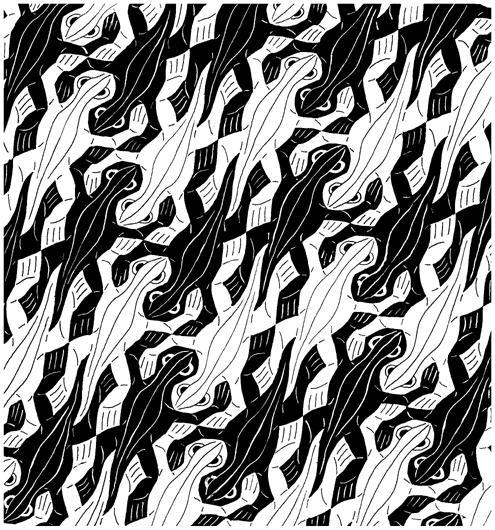
\includegraphics[height=4.8cm]{tess5}}
  \subfloat[]{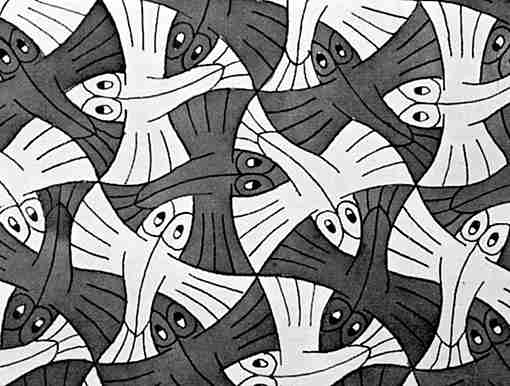
\includegraphics[height=4.8cm]{escher2}}
  \subfloat[]{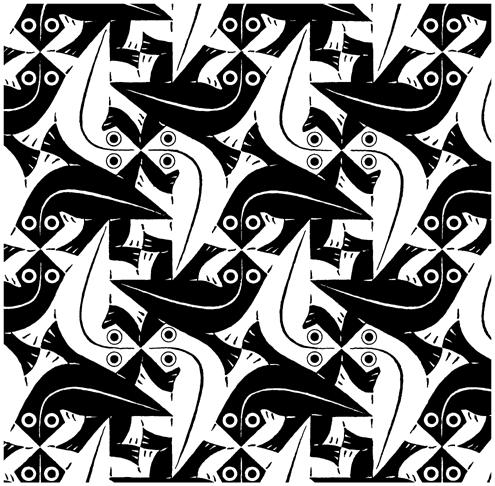
\includegraphics[height=4.8cm]{tess104}}\\
\end{figure}\\
Op deze drie afbeeldingen zien we vlakvullingen van Escher. Hier zullen we later nog op ingaan.\\
We zullen nu zelf op zoek gaan naar figuren om een vlak te vullen.

\ask{Welke eenvoudige meetkundige vlakke figuren kennen jullie?}

\answer[1cm]{Rechthoek, vierkant, driehoek, cirkel, \ldots}

\teacher{De leerlingen kunnen hier veel verschillende antwoorden geven, maar zullen waarschijnlijk wel komen tot de bovenstaande antwoorden.}

We zullen nu eens kijken hoe we een vlak volledig kunnen vullen met deze figuren aan de hand van translaties en/of rotaties. In theorie kunnen we een vlak vullen met verschillende soorten figuren, maar om het eenvoudig te houden zullen we in dit lessenpakket kijken hoe we een vlak kunnen vullen met identieke figuren.

\ask{Welke beperkingen moeten nog opleggen opdat iets een vlakvulling is? Als we nu het vlak willen vullen met identieke figuren mogen deze figuren dan overlappen?}

\answer[1cm]{}

\teacher{Laat eerst zelf vragen en opmerkingen opkomen bij de leerlingen De leerlingen kunnen ook redeneren waarom dit zo is.}

\task{Geef nu een definitie van een vlakvulling:}

\answer[2cm]{Een \textbf{vlakvulling} is een vulling van het vlak met figuren, waarbij er geen gaten mogen zijn en de figuren niet mogen overlappen.}

We kunnen nu proberen om een oneindig groot vlak zo optimaal mogelijk te vullen met identieke figuren.

\ask{Is het altijd mogelijk om een oneindig groot vlak compleet te vullen?}

\answer[1cm]{Neen}

Daarom maken we dus het onderscheid tussen twee definities. Enerzijds zullen we spreken over een \textbf{complete vlakvulling} als we een oneindig vlak volledig kunnen vullen met een bepaalde figuur aan de hand van translaties en/of rotaties. Anderzijds zullen we spreken over een \textbf{optimale vlakvulling} als we het oneindig grote vlak zo compleet mogelijk kunnen vullen. Bij optimale vlakvullingen zullen we ook spreken over de \textbf{effici\"{e}ntie} van de vlakvulling. Deze effici\"{e}ntie drukken we uit in een percentage. Als de effici\"{e}ntie van de optimale vlakvulling dus gelijk is aan $100\%$, dan hebben we een complete vlakvulling.


\subsection{Vullen van een oneindig groot vlak}

Om te beginnen kunnen we nu eens kijken hoe we een vlak compleet kunnen vullen met figuren, meer bepaald zullen we proberen het vlak te vullen met regelmatige veelhoeken. Het compleet vullen van een vlak met regelmatige veelhoeken noemen we ook een regulier vlakvulling of regulier betegeling. Eerst zullen we nu eens nadenken over de volgende vragen.

\teacher{Op dit punt verdelen we de leerlingen in groepjes en delen we aan de leerlingen identieke figuren uit die uitgeknipt werden in karton. Elk groepje krijgt een stapel identieke regelmatige driehoeken, een stapel identieke regelmatige vierhoeken, een stapel identieke regelmatige vijfhoeken, een stapel identieke regelmatige zeshoeken, een stapel identieke regelmatige zevenhoeken en een stapel identieke regelmatige achthoeken.}

\task{Probeer eens uit te zoeken met welke regelmatige veelhoeken je een complete vlakvulling kan maken.}

\teacher{De leerlingen proberen in groepjes de tafels volledig te vullen met deze kartonnen regelmatige veelhoeken en zullen zo tot bevindingen komen.}

\answer[1.5cm]{Een complete vlakvulling is enkel mogelijk met regelmatige driehoeken, regelmatige vierhoeken en regelmatige zeshoeken.}

\ask{Hoe komt het dat een complete vlakvulling met andere regelmatige veelhoeken niet lukt?}

\answer[2cm]{We zien dat bij de vlakvulling met regelmatige veelhoeken de hoeken van ieder toppunt precies moeten passen omdat we anders gaten of overlappingen hebben. De grootte van de binnenhoeken van de regelmatige veelhoeken moet dus een deler zijn van 360.}

We zullen nu onze bevindingen wiskundig correct proberen te formuleren en bewijzen. Laat ons eerst een antwoord vinden op de volgende vragen.

\ask{
\begin{itemize}
\item Kan je een formule vinden voor de som van de binnenhoeken van een regelmatige $n-$hoek?\\
\item Kan je een formule vinden voor de grootte van de binnenhoeken van een regelmatige $n-$hoek?\\
\item Dus de grootte van de binnenhoeken van een regelmatige driehoek is gelijk aan? \answer{$60\degree$}\\
\item Dus de grootte van de binnenhoeken van een regelmatige vierhoek is gelijk aan? \answer{$90\degree$}\\
\item Dus de grootte van de binnenhoeken van een regelmatige vijfhoek is gelijk aan? \answer{$108\degree$}\\
\item \ldots
\end{itemize}}

\teacher{We komen tot de volgende stelling, `Als we een oneindig groot vlak compleet willen vullen met regelmatige veelhoeken dan lukt dit enkel met regelmatige driehoeken, regelmatige vierhoeken en regelmatige zeshoeken'}

\teacher{Bewijs: De som van de binnenhoeken van een $n$-hoek is $180\degree(n-2)$. Omdat een regelmatige $n$-hoek $n$ hoeken heeft is dus de grootte van \'{e}\'{e}n binnenhoek gelijk aan $\frac{180\degree(n-2)}{n} = 180\degree(1-\frac{2}{n})$. Als we $r$ regelmatige $n$-hoeken plaatsen op \'{e}\'{e}n punt, zodanig dat ze niet overlappen en geen gaten laten, dan moet de som van alle binnenhoeken gelijk zijn aan $360\degree$.\\We krijgen dus de volgende identiteit: $$r\cdot 180\degree(1-\frac{2}{n}) = 360\degree \;.$$ Dit kan vereenvoudigd worden tot $$n = \frac{2r}{r-2}\;.$$ Omdat $n$, het aantal hoekpunten van de regelmatige veelhoek, zeker positief moet zijn, volgt alvast dat $r\geq 3$. Omdat de veelhoek met het kleinste aantal hoekpunten de driehoek is, hebben we $n\geq 3$ en volgt er dus dat $r\leq 6$. Vullen we nu $r = 3, 4, 5 \mbox{ en } 6$ in, dan krijgen we $n=6,4,\frac{10}{3} \mbox{ en } 3$. Het nummer $n$ is een natuurlijk getal, dus $n= 6, 4 \mbox{ en } 3$ zijn mogelijk. Ofwel, enkel regelmatige zeshoeken, regelmatige vierhoeken of regelmatige driehoeken kunnen een oneindig groot vlak compleet opvullen.}

\begin{figure}[ht]
  \centering
  \subfloat[Regelmatige driehoeken]{\begin{tikzpicture}[line cap=round,line join=round,>=triangle 45,x=1.0cm,y=1.0cm]
\clip(0.5,0.5) rectangle (5.5,5.5);
\fill[fill=black,fill opacity=0.1] (0,0) -- (1,0) -- (0.5,0.87) -- cycle;
\fill[fill=black,fill opacity=0.1] (0.5,0.87) -- (1,0) -- (1.5,0.87) -- cycle;
\fill[fill=black,fill opacity=0.1] (1,0) -- (2,0) -- (1.5,0.87) -- cycle;
\fill[fill=black,fill opacity=0.1] (1.5,0.87) -- (2,0) -- (2.5,0.87) -- cycle;
\fill[fill=black,fill opacity=0.1] (2,0) -- (3,0) -- (2.5,0.87) -- cycle;
\fill[fill=black,fill opacity=0.1] (2.5,0.87) -- (3,0) -- (3.5,0.87) -- cycle;
\fill[fill=black,fill opacity=0.1] (3,0) -- (4,0) -- (3.5,0.87) -- cycle;
\fill[fill=black,fill opacity=0.1] (3.5,0.87) -- (4,0) -- (4.5,0.87) -- cycle;
\fill[fill=black,fill opacity=0.1] (4,0) -- (5,0) -- (4.5,0.87) -- cycle;
\fill[fill=black,fill opacity=0.1] (4.5,0.87) -- (5,0) -- (5.5,0.87) -- cycle;
\fill[fill=black,fill opacity=0.1] (5,0) -- (6,0) -- (5.5,0.87) -- cycle;
\fill[fill=black,fill opacity=0.1] (5.5,0.87) -- (6,0) -- (6.5,0.87) -- cycle;
\fill[fill=black,fill opacity=0.1] (6,0) -- (7,0) -- (6.5,0.87) -- cycle;
\fill[fill=black,fill opacity=0.1] (6.5,0.87) -- (7,0) -- (7.5,0.87) -- cycle;
\fill[fill=black,fill opacity=0.1] (7,0) -- (8,0) -- (7.5,0.87) -- cycle;
\fill[fill=black,fill opacity=0.1] (7.5,0.87) -- (8,0) -- (8.5,0.87) -- cycle;
\fill[fill=black,fill opacity=0.1] (8,0) -- (9,0) -- (8.5,0.87) -- cycle;
\fill[fill=black,fill opacity=0.1] (8.5,0.87) -- (9,0) -- (9.5,0.87) -- cycle;
\fill[fill=black,fill opacity=0.1] (9,0) -- (10,0) -- (9.5,0.87) -- cycle;
\fill[fill=black,fill opacity=0.1] (9.5,0.87) -- (10,0) -- (10.5,0.87) -- cycle;
\fill[fill=black,fill opacity=0.1] (0,1.73) -- (0.5,0.87) -- (1,1.73) -- cycle;
\fill[fill=black,fill opacity=0.1] (0.5,0.87) -- (1.5,0.87) -- (1,1.73) -- cycle;
\fill[fill=black,fill opacity=0.1] (1,1.73) -- (1.5,0.87) -- (2,1.73) -- cycle;
\fill[fill=black,fill opacity=0.1] (1.5,0.87) -- (2.5,0.87) -- (2,1.73) -- cycle;
\fill[fill=black,fill opacity=0.1] (2,1.73) -- (2.5,0.87) -- (3,1.73) -- cycle;
\fill[fill=black,fill opacity=0.1] (2.5,0.87) -- (3.5,0.87) -- (3,1.73) -- cycle;
\fill[fill=black,fill opacity=0.1] (3,1.73) -- (3.5,0.87) -- (4,1.73) -- cycle;
\fill[fill=black,fill opacity=0.1] (3.5,0.87) -- (4.5,0.87) -- (4,1.73) -- cycle;
\fill[fill=black,fill opacity=0.1] (4,1.73) -- (4.5,0.87) -- (5,1.73) -- cycle;
\fill[fill=black,fill opacity=0.1] (4.5,0.87) -- (5.5,0.87) -- (5,1.73) -- cycle;
\fill[fill=black,fill opacity=0.1] (5,1.73) -- (5.5,0.87) -- (6,1.73) -- cycle;
\fill[fill=black,fill opacity=0.1] (5.5,0.87) -- (6.5,0.87) -- (6,1.73) -- cycle;
\fill[fill=black,fill opacity=0.1] (6,1.73) -- (6.5,0.87) -- (7,1.73) -- cycle;
\fill[fill=black,fill opacity=0.1] (6.5,0.87) -- (7.5,0.87) -- (7,1.73) -- cycle;
\fill[fill=black,fill opacity=0.1] (7,1.73) -- (7.5,0.87) -- (8,1.73) -- cycle;
\fill[fill=black,fill opacity=0.1] (7.5,0.87) -- (8.5,0.87) -- (8,1.73) -- cycle;
\fill[fill=black,fill opacity=0.1] (8,1.73) -- (8.5,0.87) -- (9,1.73) -- cycle;
\fill[fill=black,fill opacity=0.1] (8.5,0.87) -- (9.5,0.87) -- (9,1.73) -- cycle;
\fill[fill=black,fill opacity=0.1] (9,1.73) -- (9.5,0.87) -- (10,1.73) -- cycle;
\fill[fill=black,fill opacity=0.1] (9.5,0.87) -- (10.5,0.87) -- (10,1.73) -- cycle;
\fill[fill=black,fill opacity=0.1] (0,1.73) -- (1,1.73) -- (0.5,2.6) -- cycle;
\fill[fill=black,fill opacity=0.1] (0.5,2.6) -- (1,1.73) -- (1.5,2.6) -- cycle;
\fill[fill=black,fill opacity=0.1] (1,1.73) -- (2,1.73) -- (1.5,2.6) -- cycle;
\fill[fill=black,fill opacity=0.1] (1.5,2.6) -- (2,1.73) -- (2.5,2.6) -- cycle;
\fill[line width=1.6pt,fill=black,fill opacity=0.25] (2,1.73) -- (3,1.73) -- (2.5,2.6) -- cycle;
\fill[fill=black,fill opacity=0.1] (2.5,2.6) -- (3,1.73) -- (3.5,2.6) -- cycle;
\fill[fill=black,fill opacity=0.1] (3,1.73) -- (4,1.73) -- (3.5,2.6) -- cycle;
\fill[fill=black,fill opacity=0.1] (3.5,2.6) -- (4,1.73) -- (4.5,2.6) -- cycle;
\fill[fill=black,fill opacity=0.1] (4,1.73) -- (5,1.73) -- (4.5,2.6) -- cycle;
\fill[fill=black,fill opacity=0.1] (4.5,2.6) -- (5,1.73) -- (5.5,2.6) -- cycle;
\fill[fill=black,fill opacity=0.1] (5,1.73) -- (6,1.73) -- (5.5,2.6) -- cycle;
\fill[fill=black,fill opacity=0.1] (5.5,2.6) -- (6,1.73) -- (6.5,2.6) -- cycle;
\fill[fill=black,fill opacity=0.1] (6,1.73) -- (7,1.73) -- (6.5,2.6) -- cycle;
\fill[fill=black,fill opacity=0.1] (6.5,2.6) -- (7,1.73) -- (7.5,2.6) -- cycle;
\fill[fill=black,fill opacity=0.1] (7,1.73) -- (8,1.73) -- (7.5,2.6) -- cycle;
\fill[fill=black,fill opacity=0.1] (7.5,2.6) -- (8,1.73) -- (8.5,2.6) -- cycle;
\fill[fill=black,fill opacity=0.1] (8,1.73) -- (9,1.73) -- (8.5,2.6) -- cycle;
\fill[fill=black,fill opacity=0.1] (8.5,2.6) -- (9,1.73) -- (9.5,2.6) -- cycle;
\fill[fill=black,fill opacity=0.1] (9,1.73) -- (10,1.73) -- (9.5,2.6) -- cycle;
\fill[fill=black,fill opacity=0.1] (9.5,2.6) -- (10,1.73) -- (10.5,2.6) -- cycle;
\fill[fill=black,fill opacity=0.1] (0,3.46) -- (0.5,2.6) -- (1,3.46) -- cycle;
\fill[fill=black,fill opacity=0.1] (0.5,2.6) -- (1.5,2.6) -- (1,3.46) -- cycle;
\fill[fill=black,fill opacity=0.1] (1,3.46) -- (1.5,2.6) -- (2,3.46) -- cycle;
\fill[fill=black,fill opacity=0.1] (1.5,2.6) -- (2.5,2.6) -- (2,3.46) -- cycle;
\fill[fill=black,fill opacity=0.1] (2,3.46) -- (2.5,2.6) -- (3,3.46) -- cycle;
\fill[fill=black,fill opacity=0.1] (2.5,2.6) -- (3.5,2.6) -- (3,3.46) -- cycle;
\fill[fill=black,fill opacity=0.1] (3,3.46) -- (3.5,2.6) -- (4,3.46) -- cycle;
\fill[fill=black,fill opacity=0.1] (3.5,2.6) -- (4.5,2.6) -- (4,3.46) -- cycle;
\fill[fill=black,fill opacity=0.1] (4,3.46) -- (4.5,2.6) -- (5,3.46) -- cycle;
\fill[fill=black,fill opacity=0.1] (4.5,2.6) -- (5.5,2.6) -- (5,3.46) -- cycle;
\fill[fill=black,fill opacity=0.1] (5,3.46) -- (5.5,2.6) -- (6,3.46) -- cycle;
\fill[fill=black,fill opacity=0.1] (5.5,2.6) -- (6.5,2.6) -- (6,3.46) -- cycle;
\fill[fill=black,fill opacity=0.1] (6,3.46) -- (6.5,2.6) -- (7,3.46) -- cycle;
\fill[fill=black,fill opacity=0.1] (6.5,2.6) -- (7.5,2.6) -- (7,3.46) -- cycle;
\fill[fill=black,fill opacity=0.1] (7,3.46) -- (7.5,2.6) -- (8,3.46) -- cycle;
\fill[fill=black,fill opacity=0.1] (7.5,2.6) -- (8.5,2.6) -- (8,3.46) -- cycle;
\fill[fill=black,fill opacity=0.1] (8,3.46) -- (8.5,2.6) -- (9,3.46) -- cycle;
\fill[fill=black,fill opacity=0.1] (8.5,2.6) -- (9.5,2.6) -- (9,3.46) -- cycle;
\fill[fill=black,fill opacity=0.1] (9,3.46) -- (9.5,2.6) -- (10,3.46) -- cycle;
\fill[fill=black,fill opacity=0.1] (9.5,2.6) -- (10.5,2.6) -- (10,3.46) -- cycle;
\fill[fill=black,fill opacity=0.1] (0,3.46) -- (1,3.46) -- (0.5,4.33) -- cycle;
\fill[fill=black,fill opacity=0.1] (0.5,4.33) -- (1,3.46) -- (1.5,4.33) -- cycle;
\fill[fill=black,fill opacity=0.1] (1,3.46) -- (2,3.46) -- (1.5,4.33) -- cycle;
\fill[fill=black,fill opacity=0.1] (1.5,4.33) -- (2,3.46) -- (2.5,4.33) -- cycle;
\fill[fill=black,fill opacity=0.1] (2,3.46) -- (3,3.46) -- (2.5,4.33) -- cycle;
\fill[fill=black,fill opacity=0.1] (2.5,4.33) -- (3,3.46) -- (3.5,4.33) -- cycle;
\fill[fill=black,fill opacity=0.1] (3,3.46) -- (4,3.46) -- (3.5,4.33) -- cycle;
\fill[fill=black,fill opacity=0.1] (3.5,4.33) -- (4,3.46) -- (4.5,4.33) -- cycle;
\fill[fill=black,fill opacity=0.1] (4,3.46) -- (5,3.46) -- (4.5,4.33) -- cycle;
\fill[fill=black,fill opacity=0.1] (4.5,4.33) -- (5,3.46) -- (5.5,4.33) -- cycle;
\fill[fill=black,fill opacity=0.1] (5,3.46) -- (6,3.46) -- (5.5,4.33) -- cycle;
\fill[fill=black,fill opacity=0.1] (5.5,4.33) -- (6,3.46) -- (6.5,4.33) -- cycle;
\fill[fill=black,fill opacity=0.1] (6,3.46) -- (7,3.46) -- (6.5,4.33) -- cycle;
\fill[fill=black,fill opacity=0.1] (6.5,4.33) -- (7,3.46) -- (7.5,4.33) -- cycle;
\fill[fill=black,fill opacity=0.1] (7,3.46) -- (8,3.46) -- (7.5,4.33) -- cycle;
\fill[fill=black,fill opacity=0.1] (7.5,4.33) -- (8,3.46) -- (8.5,4.33) -- cycle;
\fill[fill=black,fill opacity=0.1] (8,3.46) -- (9,3.46) -- (8.5,4.33) -- cycle;
\fill[fill=black,fill opacity=0.1] (8.5,4.33) -- (9,3.46) -- (9.5,4.33) -- cycle;
\fill[fill=black,fill opacity=0.1] (9,3.46) -- (10,3.46) -- (9.5,4.33) -- cycle;
\fill[fill=black,fill opacity=0.1] (9.5,4.33) -- (10,3.46) -- (10.5,4.33) -- cycle;
\fill[fill=black,fill opacity=0.1] (0,5.2) -- (0.5,4.33) -- (1,5.2) -- cycle;
\fill[fill=black,fill opacity=0.1] (0.5,4.33) -- (1.5,4.33) -- (1,5.2) -- cycle;
\fill[fill=black,fill opacity=0.1] (1,5.2) -- (1.5,4.33) -- (2,5.2) -- cycle;
\fill[fill=black,fill opacity=0.1] (1.5,4.33) -- (2.5,4.33) -- (2,5.2) -- cycle;
\fill[fill=black,fill opacity=0.1] (2,5.2) -- (2.5,4.33) -- (3,5.2) -- cycle;
\fill[fill=black,fill opacity=0.1] (2.5,4.33) -- (3.5,4.33) -- (3,5.2) -- cycle;
\fill[fill=black,fill opacity=0.1] (3,5.2) -- (3.5,4.33) -- (4,5.2) -- cycle;
\fill[fill=black,fill opacity=0.1] (3.5,4.33) -- (4.5,4.33) -- (4,5.2) -- cycle;
\fill[fill=black,fill opacity=0.1] (4,5.2) -- (4.5,4.33) -- (5,5.2) -- cycle;
\fill[fill=black,fill opacity=0.1] (4.5,4.33) -- (5.5,4.33) -- (5,5.2) -- cycle;
\fill[fill=black,fill opacity=0.1] (5,5.2) -- (5.5,4.33) -- (6,5.2) -- cycle;
\fill[fill=black,fill opacity=0.1] (5.5,4.33) -- (6.5,4.33) -- (6,5.2) -- cycle;
\fill[fill=black,fill opacity=0.1] (6,5.2) -- (6.5,4.33) -- (7,5.2) -- cycle;
\fill[fill=black,fill opacity=0.1] (6.5,4.33) -- (7.5,4.33) -- (7,5.2) -- cycle;
\fill[fill=black,fill opacity=0.1] (7,5.2) -- (7.5,4.33) -- (8,5.2) -- cycle;
\fill[fill=black,fill opacity=0.1] (7.5,4.33) -- (8.5,4.33) -- (8,5.2) -- cycle;
\fill[fill=black,fill opacity=0.1] (8,5.2) -- (8.5,4.33) -- (9,5.2) -- cycle;
\fill[fill=black,fill opacity=0.1] (8.5,4.33) -- (9.5,4.33) -- (9,5.2) -- cycle;
\fill[fill=black,fill opacity=0.1] (9,5.2) -- (9.5,4.33) -- (10,5.2) -- cycle;
\fill[fill=black,fill opacity=0.1] (9.5,4.33) -- (10.5,4.33) -- (10,5.2) -- cycle;
\fill[fill=black,fill opacity=0.1] (0,5.2) -- (1,5.2) -- (0.5,6.06) -- cycle;
\fill[fill=black,fill opacity=0.1] (0.5,6.06) -- (1,5.2) -- (1.5,6.06) -- cycle;
\fill[fill=black,fill opacity=0.1] (1,5.2) -- (2,5.2) -- (1.5,6.06) -- cycle;
\fill[fill=black,fill opacity=0.1] (1.5,6.06) -- (2,5.2) -- (2.5,6.06) -- cycle;
\fill[fill=black,fill opacity=0.1] (2,5.2) -- (3,5.2) -- (2.5,6.06) -- cycle;
\fill[fill=black,fill opacity=0.1] (2.5,6.06) -- (3,5.2) -- (3.5,6.06) -- cycle;
\fill[fill=black,fill opacity=0.1] (3,5.2) -- (4,5.2) -- (3.5,6.06) -- cycle;
\fill[fill=black,fill opacity=0.1] (3.5,6.06) -- (4,5.2) -- (4.5,6.06) -- cycle;
\fill[fill=black,fill opacity=0.1] (4,5.2) -- (5,5.2) -- (4.5,6.06) -- cycle;
\fill[fill=black,fill opacity=0.1] (4.5,6.06) -- (5,5.2) -- (5.5,6.06) -- cycle;
\fill[fill=black,fill opacity=0.1] (5,5.2) -- (6,5.2) -- (5.5,6.06) -- cycle;
\fill[fill=black,fill opacity=0.1] (5.5,6.06) -- (6,5.2) -- (6.5,6.06) -- cycle;
\fill[fill=black,fill opacity=0.1] (6,5.2) -- (7,5.2) -- (6.5,6.06) -- cycle;
\fill[fill=black,fill opacity=0.1] (6.5,6.06) -- (7,5.2) -- (7.5,6.06) -- cycle;
\fill[fill=black,fill opacity=0.1] (7,5.2) -- (8,5.2) -- (7.5,6.06) -- cycle;
\fill[fill=black,fill opacity=0.1] (7.5,6.06) -- (8,5.2) -- (8.5,6.06) -- cycle;
\fill[fill=black,fill opacity=0.1] (8,5.2) -- (9,5.2) -- (8.5,6.06) -- cycle;
\fill[fill=black,fill opacity=0.1] (8.5,6.06) -- (9,5.2) -- (9.5,6.06) -- cycle;
\fill[fill=black,fill opacity=0.1] (9,5.2) -- (10,5.2) -- (9.5,6.06) -- cycle;
\fill[fill=black,fill opacity=0.1] (9.5,6.06) -- (10,5.2) -- (10.5,6.06) -- cycle;
\fill[fill=black,fill opacity=0.1] (0,6.93) -- (0.5,6.06) -- (1,6.93) -- cycle;
\fill[fill=black,fill opacity=0.1] (0.5,6.06) -- (1.5,6.06) -- (1,6.93) -- cycle;
\fill[fill=black,fill opacity=0.1] (1,6.93) -- (1.5,6.06) -- (2,6.93) -- cycle;
\fill[fill=black,fill opacity=0.1] (1.5,6.06) -- (2.5,6.06) -- (2,6.93) -- cycle;
\fill[fill=black,fill opacity=0.1] (2,6.93) -- (2.5,6.06) -- (3,6.93) -- cycle;
\fill[fill=black,fill opacity=0.1] (2.5,6.06) -- (3.5,6.06) -- (3,6.93) -- cycle;
\fill[fill=black,fill opacity=0.1] (3,6.93) -- (3.5,6.06) -- (4,6.93) -- cycle;
\fill[fill=black,fill opacity=0.1] (3.5,6.06) -- (4.5,6.06) -- (4,6.93) -- cycle;
\fill[fill=black,fill opacity=0.1] (4,6.93) -- (4.5,6.06) -- (5,6.93) -- cycle;
\fill[fill=black,fill opacity=0.1] (4.5,6.06) -- (5.5,6.06) -- (5,6.93) -- cycle;
\fill[fill=black,fill opacity=0.1] (5,6.93) -- (5.5,6.06) -- (6,6.93) -- cycle;
\fill[fill=black,fill opacity=0.1] (5.5,6.06) -- (6.5,6.06) -- (6,6.93) -- cycle;
\fill[fill=black,fill opacity=0.1] (6,6.93) -- (6.5,6.06) -- (7,6.93) -- cycle;
\fill[fill=black,fill opacity=0.1] (6.5,6.06) -- (7.5,6.06) -- (7,6.93) -- cycle;
\fill[fill=black,fill opacity=0.1] (7,6.93) -- (7.5,6.06) -- (8,6.93) -- cycle;
\fill[fill=black,fill opacity=0.1] (7.5,6.06) -- (8.5,6.06) -- (8,6.93) -- cycle;
\fill[fill=black,fill opacity=0.1] (8,6.93) -- (8.5,6.06) -- (9,6.93) -- cycle;
\fill[fill=black,fill opacity=0.1] (8.5,6.06) -- (9.5,6.06) -- (9,6.93) -- cycle;
\fill[fill=black,fill opacity=0.1] (9,6.93) -- (9.5,6.06) -- (10,6.93) -- cycle;
\fill[fill=black,fill opacity=0.1] (9.5,6.06) -- (10.5,6.06) -- (10,6.93) -- cycle;
\fill[fill=black,fill opacity=0.1] (0,6.93) -- (1,6.93) -- (0.5,7.79) -- cycle;
\fill[fill=black,fill opacity=0.1] (0.5,7.79) -- (1,6.93) -- (1.5,7.79) -- cycle;
\fill[fill=black,fill opacity=0.1] (1,6.93) -- (2,6.93) -- (1.5,7.79) -- cycle;
\fill[fill=black,fill opacity=0.1] (1.5,7.79) -- (2,6.93) -- (2.5,7.79) -- cycle;
\fill[fill=black,fill opacity=0.1] (2,6.93) -- (3,6.93) -- (2.5,7.79) -- cycle;
\fill[fill=black,fill opacity=0.1] (2.5,7.79) -- (3,6.93) -- (3.5,7.79) -- cycle;
\fill[fill=black,fill opacity=0.1] (3,6.93) -- (4,6.93) -- (3.5,7.79) -- cycle;
\fill[fill=black,fill opacity=0.1] (3.5,7.79) -- (4,6.93) -- (4.5,7.79) -- cycle;
\fill[fill=black,fill opacity=0.1] (4,6.93) -- (5,6.93) -- (4.5,7.79) -- cycle;
\fill[fill=black,fill opacity=0.1] (4.5,7.79) -- (5,6.93) -- (5.5,7.79) -- cycle;
\fill[fill=black,fill opacity=0.1] (5,6.93) -- (6,6.93) -- (5.5,7.79) -- cycle;
\fill[fill=black,fill opacity=0.1] (5.5,7.79) -- (6,6.93) -- (6.5,7.79) -- cycle;
\fill[fill=black,fill opacity=0.1] (6,6.93) -- (7,6.93) -- (6.5,7.79) -- cycle;
\fill[fill=black,fill opacity=0.1] (6.5,7.79) -- (7,6.93) -- (7.5,7.79) -- cycle;
\fill[fill=black,fill opacity=0.1] (7,6.93) -- (8,6.93) -- (7.5,7.79) -- cycle;
\fill[fill=black,fill opacity=0.1] (7.5,7.79) -- (8,6.93) -- (8.5,7.79) -- cycle;
\fill[fill=black,fill opacity=0.1] (8,6.93) -- (9,6.93) -- (8.5,7.79) -- cycle;
\fill[fill=black,fill opacity=0.1] (8.5,7.79) -- (9,6.93) -- (9.5,7.79) -- cycle;
\fill[fill=black,fill opacity=0.1] (9,6.93) -- (10,6.93) -- (9.5,7.79) -- cycle;
\fill[fill=black,fill opacity=0.1] (9.5,7.79) -- (10,6.93) -- (10.5,7.79) -- cycle;
\fill[fill=black,fill opacity=0.1] (0,8.66) -- (0.5,7.79) -- (1,8.66) -- cycle;
\fill[fill=black,fill opacity=0.1] (0.5,7.79) -- (1.5,7.79) -- (1,8.66) -- cycle;
\fill[fill=black,fill opacity=0.1] (1,8.66) -- (1.5,7.79) -- (2,8.66) -- cycle;
\fill[fill=black,fill opacity=0.1] (1.5,7.79) -- (2.5,7.79) -- (2,8.66) -- cycle;
\fill[fill=black,fill opacity=0.1] (2,8.66) -- (2.5,7.79) -- (3,8.66) -- cycle;
\fill[fill=black,fill opacity=0.1] (2.5,7.79) -- (3.5,7.79) -- (3,8.66) -- cycle;
\fill[fill=black,fill opacity=0.1] (3,8.66) -- (3.5,7.79) -- (4,8.66) -- cycle;
\fill[fill=black,fill opacity=0.1] (3.5,7.79) -- (4.5,7.79) -- (4,8.66) -- cycle;
\fill[fill=black,fill opacity=0.1] (4,8.66) -- (4.5,7.79) -- (5,8.66) -- cycle;
\fill[fill=black,fill opacity=0.1] (4.5,7.79) -- (5.5,7.79) -- (5,8.66) -- cycle;
\fill[fill=black,fill opacity=0.1] (5,8.66) -- (5.5,7.79) -- (6,8.66) -- cycle;
\fill[fill=black,fill opacity=0.1] (5.5,7.79) -- (6.5,7.79) -- (6,8.66) -- cycle;
\fill[fill=black,fill opacity=0.1] (6,8.66) -- (6.5,7.79) -- (7,8.66) -- cycle;
\fill[fill=black,fill opacity=0.1] (6.5,7.79) -- (7.5,7.79) -- (7,8.66) -- cycle;
\fill[fill=black,fill opacity=0.1] (7,8.66) -- (7.5,7.79) -- (8,8.66) -- cycle;
\fill[fill=black,fill opacity=0.1] (7.5,7.79) -- (8.5,7.79) -- (8,8.66) -- cycle;
\fill[fill=black,fill opacity=0.1] (8,8.66) -- (8.5,7.79) -- (9,8.66) -- cycle;
\fill[fill=black,fill opacity=0.1] (8.5,7.79) -- (9.5,7.79) -- (9,8.66) -- cycle;
\fill[fill=black,fill opacity=0.1] (9,8.66) -- (9.5,7.79) -- (10,8.66) -- cycle;
\fill[fill=black,fill opacity=0.1] (9.5,7.79) -- (10.5,7.79) -- (10,8.66) -- cycle;
\fill[fill=black,fill opacity=0.1] (0,8.66) -- (1,8.66) -- (0.5,9.53) -- cycle;
\fill[fill=black,fill opacity=0.1] (0.5,9.53) -- (1,8.66) -- (1.5,9.53) -- cycle;
\fill[fill=black,fill opacity=0.1] (1,8.66) -- (2,8.66) -- (1.5,9.53) -- cycle;
\fill[fill=black,fill opacity=0.1] (1.5,9.53) -- (2,8.66) -- (2.5,9.53) -- cycle;
\fill[fill=black,fill opacity=0.1] (2,8.66) -- (3,8.66) -- (2.5,9.53) -- cycle;
\fill[fill=black,fill opacity=0.1] (2.5,9.53) -- (3,8.66) -- (3.5,9.53) -- cycle;
\fill[fill=black,fill opacity=0.1] (3,8.66) -- (4,8.66) -- (3.5,9.53) -- cycle;
\fill[fill=black,fill opacity=0.1] (3.5,9.53) -- (4,8.66) -- (4.5,9.53) -- cycle;
\fill[fill=black,fill opacity=0.1] (4,8.66) -- (5,8.66) -- (4.5,9.53) -- cycle;
\fill[fill=black,fill opacity=0.1] (4.5,9.53) -- (5,8.66) -- (5.5,9.53) -- cycle;
\fill[fill=black,fill opacity=0.1] (5,8.66) -- (6,8.66) -- (5.5,9.53) -- cycle;
\fill[fill=black,fill opacity=0.1] (5.5,9.53) -- (6,8.66) -- (6.5,9.53) -- cycle;
\fill[fill=black,fill opacity=0.1] (6,8.66) -- (7,8.66) -- (6.5,9.53) -- cycle;
\fill[fill=black,fill opacity=0.1] (6.5,9.53) -- (7,8.66) -- (7.5,9.53) -- cycle;
\fill[fill=black,fill opacity=0.1] (7,8.66) -- (8,8.66) -- (7.5,9.53) -- cycle;
\fill[fill=black,fill opacity=0.1] (7.5,9.53) -- (8,8.66) -- (8.5,9.53) -- cycle;
\fill[fill=black,fill opacity=0.1] (8,8.66) -- (9,8.66) -- (8.5,9.53) -- cycle;
\fill[fill=black,fill opacity=0.1] (8.5,9.53) -- (9,8.66) -- (9.5,9.53) -- cycle;
\fill[fill=black,fill opacity=0.1] (9,8.66) -- (10,8.66) -- (9.5,9.53) -- cycle;
\fill[fill=black,fill opacity=0.1] (9.5,9.53) -- (10,8.66) -- (10.5,9.53) -- cycle;
\fill[fill=black,fill opacity=0.1] (0,10.39) -- (0.5,9.53) -- (1,10.39) -- cycle;
\fill[fill=black,fill opacity=0.1] (0.5,9.53) -- (1.5,9.53) -- (1,10.39) -- cycle;
\fill[fill=black,fill opacity=0.1] (1,10.39) -- (1.5,9.53) -- (2,10.39) -- cycle;
\fill[fill=black,fill opacity=0.1] (1.5,9.53) -- (2.5,9.53) -- (2,10.39) -- cycle;
\fill[fill=black,fill opacity=0.1] (2,10.39) -- (2.5,9.53) -- (3,10.39) -- cycle;
\fill[fill=black,fill opacity=0.1] (2.5,9.53) -- (3.5,9.53) -- (3,10.39) -- cycle;
\fill[fill=black,fill opacity=0.1] (3,10.39) -- (3.5,9.53) -- (4,10.39) -- cycle;
\fill[fill=black,fill opacity=0.1] (3.5,9.53) -- (4.5,9.53) -- (4,10.39) -- cycle;
\fill[fill=black,fill opacity=0.1] (4,10.39) -- (4.5,9.53) -- (5,10.39) -- cycle;
\fill[fill=black,fill opacity=0.1] (4.5,9.53) -- (5.5,9.53) -- (5,10.39) -- cycle;
\fill[fill=black,fill opacity=0.1] (5,10.39) -- (5.5,9.53) -- (6,10.39) -- cycle;
\fill[fill=black,fill opacity=0.1] (5.5,9.53) -- (6.5,9.53) -- (6,10.39) -- cycle;
\fill[fill=black,fill opacity=0.1] (6,10.39) -- (6.5,9.53) -- (7,10.39) -- cycle;
\fill[fill=black,fill opacity=0.1] (6.5,9.53) -- (7.5,9.53) -- (7,10.39) -- cycle;
\fill[fill=black,fill opacity=0.1] (7,10.39) -- (7.5,9.53) -- (8,10.39) -- cycle;
\fill[fill=black,fill opacity=0.1] (7.5,9.53) -- (8.5,9.53) -- (8,10.39) -- cycle;
\fill[fill=black,fill opacity=0.1] (8,10.39) -- (8.5,9.53) -- (9,10.39) -- cycle;
\fill[fill=black,fill opacity=0.1] (8.5,9.53) -- (9.5,9.53) -- (9,10.39) -- cycle;
\fill[fill=black,fill opacity=0.1] (9,10.39) -- (9.5,9.53) -- (10,10.39) -- cycle;
\fill[fill=black,fill opacity=0.1] (9.5,9.53) -- (10.5,9.53) -- (10,10.39) -- cycle;
\draw (0,0)-- (1,0);
\draw (1,0)-- (0.5,0.87);
\draw (0.5,0.87)-- (0,0);
\draw (0.5,0.87)-- (1,0);
\draw (1,0)-- (1.5,0.87);
\draw (1.5,0.87)-- (0.5,0.87);
\draw (1,0)-- (2,0);
\draw (2,0)-- (1.5,0.87);
\draw (1.5,0.87)-- (1,0);
\draw (1.5,0.87)-- (2,0);
\draw (2,0)-- (2.5,0.87);
\draw (2.5,0.87)-- (1.5,0.87);
\draw (2,0)-- (3,0);
\draw (3,0)-- (2.5,0.87);
\draw (2.5,0.87)-- (2,0);
\draw (2.5,0.87)-- (3,0);
\draw (3,0)-- (3.5,0.87);
\draw (3.5,0.87)-- (2.5,0.87);
\draw (3,0)-- (4,0);
\draw (4,0)-- (3.5,0.87);
\draw (3.5,0.87)-- (3,0);
\draw (3.5,0.87)-- (4,0);
\draw (4,0)-- (4.5,0.87);
\draw (4.5,0.87)-- (3.5,0.87);
\draw (4,0)-- (5,0);
\draw (5,0)-- (4.5,0.87);
\draw (4.5,0.87)-- (4,0);
\draw (4.5,0.87)-- (5,0);
\draw (5,0)-- (5.5,0.87);
\draw (5.5,0.87)-- (4.5,0.87);
\draw (5,0)-- (6,0);
\draw (6,0)-- (5.5,0.87);
\draw (5.5,0.87)-- (5,0);
\draw (5.5,0.87)-- (6,0);
\draw (6,0)-- (6.5,0.87);
\draw (6.5,0.87)-- (5.5,0.87);
\draw (6,0)-- (7,0);
\draw (7,0)-- (6.5,0.87);
\draw (6.5,0.87)-- (6,0);
\draw (6.5,0.87)-- (7,0);
\draw (7,0)-- (7.5,0.87);
\draw (7.5,0.87)-- (6.5,0.87);
\draw (7,0)-- (8,0);
\draw (8,0)-- (7.5,0.87);
\draw (7.5,0.87)-- (7,0);
\draw (7.5,0.87)-- (8,0);
\draw (8,0)-- (8.5,0.87);
\draw (8.5,0.87)-- (7.5,0.87);
\draw (8,0)-- (9,0);
\draw (9,0)-- (8.5,0.87);
\draw (8.5,0.87)-- (8,0);
\draw (8.5,0.87)-- (9,0);
\draw (9,0)-- (9.5,0.87);
\draw (9.5,0.87)-- (8.5,0.87);
\draw (9,0)-- (10,0);
\draw (10,0)-- (9.5,0.87);
\draw (9.5,0.87)-- (9,0);
\draw (9.5,0.87)-- (10,0);
\draw (10,0)-- (10.5,0.87);
\draw (10.5,0.87)-- (9.5,0.87);
\draw (0,1.73)-- (0.5,0.87);
\draw (0.5,0.87)-- (1,1.73);
\draw (1,1.73)-- (0,1.73);
\draw (0.5,0.87)-- (1.5,0.87);
\draw (1.5,0.87)-- (1,1.73);
\draw (1,1.73)-- (0.5,0.87);
\draw (1,1.73)-- (1.5,0.87);
\draw (1.5,0.87)-- (2,1.73);
\draw (2,1.73)-- (1,1.73);
\draw (1.5,0.87)-- (2.5,0.87);
\draw (2.5,0.87)-- (2,1.73);
\draw (2,1.73)-- (1.5,0.87);
\draw (2,1.73)-- (2.5,0.87);
\draw (2.5,0.87)-- (3,1.73);
\draw (3,1.73)-- (2,1.73);
\draw (2.5,0.87)-- (3.5,0.87);
\draw (3.5,0.87)-- (3,1.73);
\draw (3,1.73)-- (2.5,0.87);
\draw (3,1.73)-- (3.5,0.87);
\draw (3.5,0.87)-- (4,1.73);
\draw (4,1.73)-- (3,1.73);
\draw (3.5,0.87)-- (4.5,0.87);
\draw (4.5,0.87)-- (4,1.73);
\draw (4,1.73)-- (3.5,0.87);
\draw (4,1.73)-- (4.5,0.87);
\draw (4.5,0.87)-- (5,1.73);
\draw (5,1.73)-- (4,1.73);
\draw (4.5,0.87)-- (5.5,0.87);
\draw (5.5,0.87)-- (5,1.73);
\draw (5,1.73)-- (4.5,0.87);
\draw (5,1.73)-- (5.5,0.87);
\draw (5.5,0.87)-- (6,1.73);
\draw (6,1.73)-- (5,1.73);
\draw (5.5,0.87)-- (6.5,0.87);
\draw (6.5,0.87)-- (6,1.73);
\draw (6,1.73)-- (5.5,0.87);
\draw (6,1.73)-- (6.5,0.87);
\draw (6.5,0.87)-- (7,1.73);
\draw (7,1.73)-- (6,1.73);
\draw (6.5,0.87)-- (7.5,0.87);
\draw (7.5,0.87)-- (7,1.73);
\draw (7,1.73)-- (6.5,0.87);
\draw (7,1.73)-- (7.5,0.87);
\draw (7.5,0.87)-- (8,1.73);
\draw (8,1.73)-- (7,1.73);
\draw (7.5,0.87)-- (8.5,0.87);
\draw (8.5,0.87)-- (8,1.73);
\draw (8,1.73)-- (7.5,0.87);
\draw (8,1.73)-- (8.5,0.87);
\draw (8.5,0.87)-- (9,1.73);
\draw (9,1.73)-- (8,1.73);
\draw (8.5,0.87)-- (9.5,0.87);
\draw (9.5,0.87)-- (9,1.73);
\draw (9,1.73)-- (8.5,0.87);
\draw (9,1.73)-- (9.5,0.87);
\draw (9.5,0.87)-- (10,1.73);
\draw (10,1.73)-- (9,1.73);
\draw (9.5,0.87)-- (10.5,0.87);
\draw (10.5,0.87)-- (10,1.73);
\draw (10,1.73)-- (9.5,0.87);
\draw (0,1.73)-- (1,1.73);
\draw (1,1.73)-- (0.5,2.6);
\draw (0.5,2.6)-- (0,1.73);
\draw (0.5,2.6)-- (1,1.73);
\draw (1,1.73)-- (1.5,2.6);
\draw (1.5,2.6)-- (0.5,2.6);
\draw (1,1.73)-- (2,1.73);
\draw (2,1.73)-- (1.5,2.6);
\draw (1.5,2.6)-- (1,1.73);
\draw (1.5,2.6)-- (2,1.73);
\draw (2,1.73)-- (2.5,2.6);
\draw (2.5,2.6)-- (1.5,2.6);
\draw [line width=1.6pt] (2,1.73)-- (3,1.73);
\draw [line width=1.6pt] (3,1.73)-- (2.5,2.6);
\draw [line width=1.6pt] (2.5,2.6)-- (2,1.73);
\draw (2.5,2.6)-- (3,1.73);
\draw (3,1.73)-- (3.5,2.6);
\draw (3.5,2.6)-- (2.5,2.6);
\draw (3,1.73)-- (4,1.73);
\draw (4,1.73)-- (3.5,2.6);
\draw (3.5,2.6)-- (3,1.73);
\draw (3.5,2.6)-- (4,1.73);
\draw (4,1.73)-- (4.5,2.6);
\draw (4.5,2.6)-- (3.5,2.6);
\draw (4,1.73)-- (5,1.73);
\draw (5,1.73)-- (4.5,2.6);
\draw (4.5,2.6)-- (4,1.73);
\draw (4.5,2.6)-- (5,1.73);
\draw (5,1.73)-- (5.5,2.6);
\draw (5.5,2.6)-- (4.5,2.6);
\draw (5,1.73)-- (6,1.73);
\draw (6,1.73)-- (5.5,2.6);
\draw (5.5,2.6)-- (5,1.73);
\draw (5.5,2.6)-- (6,1.73);
\draw (6,1.73)-- (6.5,2.6);
\draw (6.5,2.6)-- (5.5,2.6);
\draw (6,1.73)-- (7,1.73);
\draw (7,1.73)-- (6.5,2.6);
\draw (6.5,2.6)-- (6,1.73);
\draw (6.5,2.6)-- (7,1.73);
\draw (7,1.73)-- (7.5,2.6);
\draw (7.5,2.6)-- (6.5,2.6);
\draw (7,1.73)-- (8,1.73);
\draw (8,1.73)-- (7.5,2.6);
\draw (7.5,2.6)-- (7,1.73);
\draw (7.5,2.6)-- (8,1.73);
\draw (8,1.73)-- (8.5,2.6);
\draw (8.5,2.6)-- (7.5,2.6);
\draw (8,1.73)-- (9,1.73);
\draw (9,1.73)-- (8.5,2.6);
\draw (8.5,2.6)-- (8,1.73);
\draw (8.5,2.6)-- (9,1.73);
\draw (9,1.73)-- (9.5,2.6);
\draw (9.5,2.6)-- (8.5,2.6);
\draw (9,1.73)-- (10,1.73);
\draw (10,1.73)-- (9.5,2.6);
\draw (9.5,2.6)-- (9,1.73);
\draw (9.5,2.6)-- (10,1.73);
\draw (10,1.73)-- (10.5,2.6);
\draw (10.5,2.6)-- (9.5,2.6);
\draw (0,3.46)-- (0.5,2.6);
\draw (0.5,2.6)-- (1,3.46);
\draw (1,3.46)-- (0,3.46);
\draw (0.5,2.6)-- (1.5,2.6);
\draw (1.5,2.6)-- (1,3.46);
\draw (1,3.46)-- (0.5,2.6);
\draw (1,3.46)-- (1.5,2.6);
\draw (1.5,2.6)-- (2,3.46);
\draw (2,3.46)-- (1,3.46);
\draw (1.5,2.6)-- (2.5,2.6);
\draw (2.5,2.6)-- (2,3.46);
\draw (2,3.46)-- (1.5,2.6);
\draw (2,3.46)-- (2.5,2.6);
\draw (2.5,2.6)-- (3,3.46);
\draw (3,3.46)-- (2,3.46);
\draw (2.5,2.6)-- (3.5,2.6);
\draw (3.5,2.6)-- (3,3.46);
\draw (3,3.46)-- (2.5,2.6);
\draw (3,3.46)-- (3.5,2.6);
\draw (3.5,2.6)-- (4,3.46);
\draw (4,3.46)-- (3,3.46);
\draw (3.5,2.6)-- (4.5,2.6);
\draw (4.5,2.6)-- (4,3.46);
\draw (4,3.46)-- (3.5,2.6);
\draw (4,3.46)-- (4.5,2.6);
\draw (4.5,2.6)-- (5,3.46);
\draw (5,3.46)-- (4,3.46);
\draw (4.5,2.6)-- (5.5,2.6);
\draw (5.5,2.6)-- (5,3.46);
\draw (5,3.46)-- (4.5,2.6);
\draw (5,3.46)-- (5.5,2.6);
\draw (5.5,2.6)-- (6,3.46);
\draw (6,3.46)-- (5,3.46);
\draw (5.5,2.6)-- (6.5,2.6);
\draw (6.5,2.6)-- (6,3.46);
\draw (6,3.46)-- (5.5,2.6);
\draw (6,3.46)-- (6.5,2.6);
\draw (6.5,2.6)-- (7,3.46);
\draw (7,3.46)-- (6,3.46);
\draw (6.5,2.6)-- (7.5,2.6);
\draw (7.5,2.6)-- (7,3.46);
\draw (7,3.46)-- (6.5,2.6);
\draw (7,3.46)-- (7.5,2.6);
\draw (7.5,2.6)-- (8,3.46);
\draw (8,3.46)-- (7,3.46);
\draw (7.5,2.6)-- (8.5,2.6);
\draw (8.5,2.6)-- (8,3.46);
\draw (8,3.46)-- (7.5,2.6);
\draw (8,3.46)-- (8.5,2.6);
\draw (8.5,2.6)-- (9,3.46);
\draw (9,3.46)-- (8,3.46);
\draw (8.5,2.6)-- (9.5,2.6);
\draw (9.5,2.6)-- (9,3.46);
\draw (9,3.46)-- (8.5,2.6);
\draw (9,3.46)-- (9.5,2.6);
\draw (9.5,2.6)-- (10,3.46);
\draw (10,3.46)-- (9,3.46);
\draw (9.5,2.6)-- (10.5,2.6);
\draw (10.5,2.6)-- (10,3.46);
\draw (10,3.46)-- (9.5,2.6);
\draw (0,3.46)-- (1,3.46);
\draw (1,3.46)-- (0.5,4.33);
\draw (0.5,4.33)-- (0,3.46);
\draw (0.5,4.33)-- (1,3.46);
\draw (1,3.46)-- (1.5,4.33);
\draw (1.5,4.33)-- (0.5,4.33);
\draw (1,3.46)-- (2,3.46);
\draw (2,3.46)-- (1.5,4.33);
\draw (1.5,4.33)-- (1,3.46);
\draw (1.5,4.33)-- (2,3.46);
\draw (2,3.46)-- (2.5,4.33);
\draw (2.5,4.33)-- (1.5,4.33);
\draw (2,3.46)-- (3,3.46);
\draw (3,3.46)-- (2.5,4.33);
\draw (2.5,4.33)-- (2,3.46);
\draw (2.5,4.33)-- (3,3.46);
\draw (3,3.46)-- (3.5,4.33);
\draw (3.5,4.33)-- (2.5,4.33);
\draw (3,3.46)-- (4,3.46);
\draw (4,3.46)-- (3.5,4.33);
\draw (3.5,4.33)-- (3,3.46);
\draw (3.5,4.33)-- (4,3.46);
\draw (4,3.46)-- (4.5,4.33);
\draw (4.5,4.33)-- (3.5,4.33);
\draw (4,3.46)-- (5,3.46);
\draw (5,3.46)-- (4.5,4.33);
\draw (4.5,4.33)-- (4,3.46);
\draw (4.5,4.33)-- (5,3.46);
\draw (5,3.46)-- (5.5,4.33);
\draw (5.5,4.33)-- (4.5,4.33);
\draw (5,3.46)-- (6,3.46);
\draw (6,3.46)-- (5.5,4.33);
\draw (5.5,4.33)-- (5,3.46);
\draw (5.5,4.33)-- (6,3.46);
\draw (6,3.46)-- (6.5,4.33);
\draw (6.5,4.33)-- (5.5,4.33);
\draw (6,3.46)-- (7,3.46);
\draw (7,3.46)-- (6.5,4.33);
\draw (6.5,4.33)-- (6,3.46);
\draw (6.5,4.33)-- (7,3.46);
\draw (7,3.46)-- (7.5,4.33);
\draw (7.5,4.33)-- (6.5,4.33);
\draw (7,3.46)-- (8,3.46);
\draw (8,3.46)-- (7.5,4.33);
\draw (7.5,4.33)-- (7,3.46);
\draw (7.5,4.33)-- (8,3.46);
\draw (8,3.46)-- (8.5,4.33);
\draw (8.5,4.33)-- (7.5,4.33);
\draw (8,3.46)-- (9,3.46);
\draw (9,3.46)-- (8.5,4.33);
\draw (8.5,4.33)-- (8,3.46);
\draw (8.5,4.33)-- (9,3.46);
\draw (9,3.46)-- (9.5,4.33);
\draw (9.5,4.33)-- (8.5,4.33);
\draw (9,3.46)-- (10,3.46);
\draw (10,3.46)-- (9.5,4.33);
\draw (9.5,4.33)-- (9,3.46);
\draw (9.5,4.33)-- (10,3.46);
\draw (10,3.46)-- (10.5,4.33);
\draw (10.5,4.33)-- (9.5,4.33);
\draw (0,5.2)-- (0.5,4.33);
\draw (0.5,4.33)-- (1,5.2);
\draw (1,5.2)-- (0,5.2);
\draw (0.5,4.33)-- (1.5,4.33);
\draw (1.5,4.33)-- (1,5.2);
\draw (1,5.2)-- (0.5,4.33);
\draw (1,5.2)-- (1.5,4.33);
\draw (1.5,4.33)-- (2,5.2);
\draw (2,5.2)-- (1,5.2);
\draw (1.5,4.33)-- (2.5,4.33);
\draw (2.5,4.33)-- (2,5.2);
\draw (2,5.2)-- (1.5,4.33);
\draw (2,5.2)-- (2.5,4.33);
\draw (2.5,4.33)-- (3,5.2);
\draw (3,5.2)-- (2,5.2);
\draw (2.5,4.33)-- (3.5,4.33);
\draw (3.5,4.33)-- (3,5.2);
\draw (3,5.2)-- (2.5,4.33);
\draw (3,5.2)-- (3.5,4.33);
\draw (3.5,4.33)-- (4,5.2);
\draw (4,5.2)-- (3,5.2);
\draw (3.5,4.33)-- (4.5,4.33);
\draw (4.5,4.33)-- (4,5.2);
\draw (4,5.2)-- (3.5,4.33);
\draw (4,5.2)-- (4.5,4.33);
\draw (4.5,4.33)-- (5,5.2);
\draw (5,5.2)-- (4,5.2);
\draw (4.5,4.33)-- (5.5,4.33);
\draw (5.5,4.33)-- (5,5.2);
\draw (5,5.2)-- (4.5,4.33);
\draw (5,5.2)-- (5.5,4.33);
\draw (5.5,4.33)-- (6,5.2);
\draw (6,5.2)-- (5,5.2);
\draw (5.5,4.33)-- (6.5,4.33);
\draw (6.5,4.33)-- (6,5.2);
\draw (6,5.2)-- (5.5,4.33);
\draw (6,5.2)-- (6.5,4.33);
\draw (6.5,4.33)-- (7,5.2);
\draw (7,5.2)-- (6,5.2);
\draw (6.5,4.33)-- (7.5,4.33);
\draw (7.5,4.33)-- (7,5.2);
\draw (7,5.2)-- (6.5,4.33);
\draw (7,5.2)-- (7.5,4.33);
\draw (7.5,4.33)-- (8,5.2);
\draw (8,5.2)-- (7,5.2);
\draw (7.5,4.33)-- (8.5,4.33);
\draw (8.5,4.33)-- (8,5.2);
\draw (8,5.2)-- (7.5,4.33);
\draw (8,5.2)-- (8.5,4.33);
\draw (8.5,4.33)-- (9,5.2);
\draw (9,5.2)-- (8,5.2);
\draw (8.5,4.33)-- (9.5,4.33);
\draw (9.5,4.33)-- (9,5.2);
\draw (9,5.2)-- (8.5,4.33);
\draw (9,5.2)-- (9.5,4.33);
\draw (9.5,4.33)-- (10,5.2);
\draw (10,5.2)-- (9,5.2);
\draw (9.5,4.33)-- (10.5,4.33);
\draw (10.5,4.33)-- (10,5.2);
\draw (10,5.2)-- (9.5,4.33);
\draw (0,5.2)-- (1,5.2);
\draw (1,5.2)-- (0.5,6.06);
\draw (0.5,6.06)-- (0,5.2);
\draw (0.5,6.06)-- (1,5.2);
\draw (1,5.2)-- (1.5,6.06);
\draw (1.5,6.06)-- (0.5,6.06);
\draw (1,5.2)-- (2,5.2);
\draw (2,5.2)-- (1.5,6.06);
\draw (1.5,6.06)-- (1,5.2);
\draw (1.5,6.06)-- (2,5.2);
\draw (2,5.2)-- (2.5,6.06);
\draw (2.5,6.06)-- (1.5,6.06);
\draw (2,5.2)-- (3,5.2);
\draw (3,5.2)-- (2.5,6.06);
\draw (2.5,6.06)-- (2,5.2);
\draw (2.5,6.06)-- (3,5.2);
\draw (3,5.2)-- (3.5,6.06);
\draw (3.5,6.06)-- (2.5,6.06);
\draw (3,5.2)-- (4,5.2);
\draw (4,5.2)-- (3.5,6.06);
\draw (3.5,6.06)-- (3,5.2);
\draw (3.5,6.06)-- (4,5.2);
\draw (4,5.2)-- (4.5,6.06);
\draw (4.5,6.06)-- (3.5,6.06);
\draw (4,5.2)-- (5,5.2);
\draw (5,5.2)-- (4.5,6.06);
\draw (4.5,6.06)-- (4,5.2);
\draw (4.5,6.06)-- (5,5.2);
\draw (5,5.2)-- (5.5,6.06);
\draw (5.5,6.06)-- (4.5,6.06);
\draw (5,5.2)-- (6,5.2);
\draw (6,5.2)-- (5.5,6.06);
\draw (5.5,6.06)-- (5,5.2);
\draw (5.5,6.06)-- (6,5.2);
\draw (6,5.2)-- (6.5,6.06);
\draw (6.5,6.06)-- (5.5,6.06);
\draw (6,5.2)-- (7,5.2);
\draw (7,5.2)-- (6.5,6.06);
\draw (6.5,6.06)-- (6,5.2);
\draw (6.5,6.06)-- (7,5.2);
\draw (7,5.2)-- (7.5,6.06);
\draw (7.5,6.06)-- (6.5,6.06);
\draw (7,5.2)-- (8,5.2);
\draw (8,5.2)-- (7.5,6.06);
\draw (7.5,6.06)-- (7,5.2);
\draw (7.5,6.06)-- (8,5.2);
\draw (8,5.2)-- (8.5,6.06);
\draw (8.5,6.06)-- (7.5,6.06);
\draw (8,5.2)-- (9,5.2);
\draw (9,5.2)-- (8.5,6.06);
\draw (8.5,6.06)-- (8,5.2);
\draw (8.5,6.06)-- (9,5.2);
\draw (9,5.2)-- (9.5,6.06);
\draw (9.5,6.06)-- (8.5,6.06);
\draw (9,5.2)-- (10,5.2);
\draw (10,5.2)-- (9.5,6.06);
\draw (9.5,6.06)-- (9,5.2);
\draw (9.5,6.06)-- (10,5.2);
\draw (10,5.2)-- (10.5,6.06);
\draw (10.5,6.06)-- (9.5,6.06);
\draw (0,6.93)-- (0.5,6.06);
\draw (0.5,6.06)-- (1,6.93);
\draw (1,6.93)-- (0,6.93);
\draw (0.5,6.06)-- (1.5,6.06);
\draw (1.5,6.06)-- (1,6.93);
\draw (1,6.93)-- (0.5,6.06);
\draw (1,6.93)-- (1.5,6.06);
\draw (1.5,6.06)-- (2,6.93);
\draw (2,6.93)-- (1,6.93);
\draw (1.5,6.06)-- (2.5,6.06);
\draw (2.5,6.06)-- (2,6.93);
\draw (2,6.93)-- (1.5,6.06);
\draw (2,6.93)-- (2.5,6.06);
\draw (2.5,6.06)-- (3,6.93);
\draw (3,6.93)-- (2,6.93);
\draw (2.5,6.06)-- (3.5,6.06);
\draw (3.5,6.06)-- (3,6.93);
\draw (3,6.93)-- (2.5,6.06);
\draw (3,6.93)-- (3.5,6.06);
\draw (3.5,6.06)-- (4,6.93);
\draw (4,6.93)-- (3,6.93);
\draw (3.5,6.06)-- (4.5,6.06);
\draw (4.5,6.06)-- (4,6.93);
\draw (4,6.93)-- (3.5,6.06);
\draw (4,6.93)-- (4.5,6.06);
\draw (4.5,6.06)-- (5,6.93);
\draw (5,6.93)-- (4,6.93);
\draw (4.5,6.06)-- (5.5,6.06);
\draw (5.5,6.06)-- (5,6.93);
\draw (5,6.93)-- (4.5,6.06);
\draw (5,6.93)-- (5.5,6.06);
\draw (5.5,6.06)-- (6,6.93);
\draw (6,6.93)-- (5,6.93);
\draw (5.5,6.06)-- (6.5,6.06);
\draw (6.5,6.06)-- (6,6.93);
\draw (6,6.93)-- (5.5,6.06);
\draw (6,6.93)-- (6.5,6.06);
\draw (6.5,6.06)-- (7,6.93);
\draw (7,6.93)-- (6,6.93);
\draw (6.5,6.06)-- (7.5,6.06);
\draw (7.5,6.06)-- (7,6.93);
\draw (7,6.93)-- (6.5,6.06);
\draw (7,6.93)-- (7.5,6.06);
\draw (7.5,6.06)-- (8,6.93);
\draw (8,6.93)-- (7,6.93);
\draw (7.5,6.06)-- (8.5,6.06);
\draw (8.5,6.06)-- (8,6.93);
\draw (8,6.93)-- (7.5,6.06);
\draw (8,6.93)-- (8.5,6.06);
\draw (8.5,6.06)-- (9,6.93);
\draw (9,6.93)-- (8,6.93);
\draw (8.5,6.06)-- (9.5,6.06);
\draw (9.5,6.06)-- (9,6.93);
\draw (9,6.93)-- (8.5,6.06);
\draw (9,6.93)-- (9.5,6.06);
\draw (9.5,6.06)-- (10,6.93);
\draw (10,6.93)-- (9,6.93);
\draw (9.5,6.06)-- (10.5,6.06);
\draw (10.5,6.06)-- (10,6.93);
\draw (10,6.93)-- (9.5,6.06);
\draw (0,6.93)-- (1,6.93);
\draw (1,6.93)-- (0.5,7.79);
\draw (0.5,7.79)-- (0,6.93);
\draw (0.5,7.79)-- (1,6.93);
\draw (1,6.93)-- (1.5,7.79);
\draw (1.5,7.79)-- (0.5,7.79);
\draw (1,6.93)-- (2,6.93);
\draw (2,6.93)-- (1.5,7.79);
\draw (1.5,7.79)-- (1,6.93);
\draw (1.5,7.79)-- (2,6.93);
\draw (2,6.93)-- (2.5,7.79);
\draw (2.5,7.79)-- (1.5,7.79);
\draw (2,6.93)-- (3,6.93);
\draw (3,6.93)-- (2.5,7.79);
\draw (2.5,7.79)-- (2,6.93);
\draw (2.5,7.79)-- (3,6.93);
\draw (3,6.93)-- (3.5,7.79);
\draw (3.5,7.79)-- (2.5,7.79);
\draw (3,6.93)-- (4,6.93);
\draw (4,6.93)-- (3.5,7.79);
\draw (3.5,7.79)-- (3,6.93);
\draw (3.5,7.79)-- (4,6.93);
\draw (4,6.93)-- (4.5,7.79);
\draw (4.5,7.79)-- (3.5,7.79);
\draw (4,6.93)-- (5,6.93);
\draw (5,6.93)-- (4.5,7.79);
\draw (4.5,7.79)-- (4,6.93);
\draw (4.5,7.79)-- (5,6.93);
\draw (5,6.93)-- (5.5,7.79);
\draw (5.5,7.79)-- (4.5,7.79);
\draw (5,6.93)-- (6,6.93);
\draw (6,6.93)-- (5.5,7.79);
\draw (5.5,7.79)-- (5,6.93);
\draw (5.5,7.79)-- (6,6.93);
\draw (6,6.93)-- (6.5,7.79);
\draw (6.5,7.79)-- (5.5,7.79);
\draw (6,6.93)-- (7,6.93);
\draw (7,6.93)-- (6.5,7.79);
\draw (6.5,7.79)-- (6,6.93);
\draw (6.5,7.79)-- (7,6.93);
\draw (7,6.93)-- (7.5,7.79);
\draw (7.5,7.79)-- (6.5,7.79);
\draw (7,6.93)-- (8,6.93);
\draw (8,6.93)-- (7.5,7.79);
\draw (7.5,7.79)-- (7,6.93);
\draw (7.5,7.79)-- (8,6.93);
\draw (8,6.93)-- (8.5,7.79);
\draw (8.5,7.79)-- (7.5,7.79);
\draw (8,6.93)-- (9,6.93);
\draw (9,6.93)-- (8.5,7.79);
\draw (8.5,7.79)-- (8,6.93);
\draw (8.5,7.79)-- (9,6.93);
\draw (9,6.93)-- (9.5,7.79);
\draw (9.5,7.79)-- (8.5,7.79);
\draw (9,6.93)-- (10,6.93);
\draw (10,6.93)-- (9.5,7.79);
\draw (9.5,7.79)-- (9,6.93);
\draw (9.5,7.79)-- (10,6.93);
\draw (10,6.93)-- (10.5,7.79);
\draw (10.5,7.79)-- (9.5,7.79);
\draw (0,8.66)-- (0.5,7.79);
\draw (0.5,7.79)-- (1,8.66);
\draw (1,8.66)-- (0,8.66);
\draw (0.5,7.79)-- (1.5,7.79);
\draw (1.5,7.79)-- (1,8.66);
\draw (1,8.66)-- (0.5,7.79);
\draw (1,8.66)-- (1.5,7.79);
\draw (1.5,7.79)-- (2,8.66);
\draw (2,8.66)-- (1,8.66);
\draw (1.5,7.79)-- (2.5,7.79);
\draw (2.5,7.79)-- (2,8.66);
\draw (2,8.66)-- (1.5,7.79);
\draw (2,8.66)-- (2.5,7.79);
\draw (2.5,7.79)-- (3,8.66);
\draw (3,8.66)-- (2,8.66);
\draw (2.5,7.79)-- (3.5,7.79);
\draw (3.5,7.79)-- (3,8.66);
\draw (3,8.66)-- (2.5,7.79);
\draw (3,8.66)-- (3.5,7.79);
\draw (3.5,7.79)-- (4,8.66);
\draw (4,8.66)-- (3,8.66);
\draw (3.5,7.79)-- (4.5,7.79);
\draw (4.5,7.79)-- (4,8.66);
\draw (4,8.66)-- (3.5,7.79);
\draw (4,8.66)-- (4.5,7.79);
\draw (4.5,7.79)-- (5,8.66);
\draw (5,8.66)-- (4,8.66);
\draw (4.5,7.79)-- (5.5,7.79);
\draw (5.5,7.79)-- (5,8.66);
\draw (5,8.66)-- (4.5,7.79);
\draw (5,8.66)-- (5.5,7.79);
\draw (5.5,7.79)-- (6,8.66);
\draw (6,8.66)-- (5,8.66);
\draw (5.5,7.79)-- (6.5,7.79);
\draw (6.5,7.79)-- (6,8.66);
\draw (6,8.66)-- (5.5,7.79);
\draw (6,8.66)-- (6.5,7.79);
\draw (6.5,7.79)-- (7,8.66);
\draw (7,8.66)-- (6,8.66);
\draw (6.5,7.79)-- (7.5,7.79);
\draw (7.5,7.79)-- (7,8.66);
\draw (7,8.66)-- (6.5,7.79);
\draw (7,8.66)-- (7.5,7.79);
\draw (7.5,7.79)-- (8,8.66);
\draw (8,8.66)-- (7,8.66);
\draw (7.5,7.79)-- (8.5,7.79);
\draw (8.5,7.79)-- (8,8.66);
\draw (8,8.66)-- (7.5,7.79);
\draw (8,8.66)-- (8.5,7.79);
\draw (8.5,7.79)-- (9,8.66);
\draw (9,8.66)-- (8,8.66);
\draw (8.5,7.79)-- (9.5,7.79);
\draw (9.5,7.79)-- (9,8.66);
\draw (9,8.66)-- (8.5,7.79);
\draw (9,8.66)-- (9.5,7.79);
\draw (9.5,7.79)-- (10,8.66);
\draw (10,8.66)-- (9,8.66);
\draw (9.5,7.79)-- (10.5,7.79);
\draw (10.5,7.79)-- (10,8.66);
\draw (10,8.66)-- (9.5,7.79);
\draw (0,8.66)-- (1,8.66);
\draw (1,8.66)-- (0.5,9.53);
\draw (0.5,9.53)-- (0,8.66);
\draw (0.5,9.53)-- (1,8.66);
\draw (1,8.66)-- (1.5,9.53);
\draw (1.5,9.53)-- (0.5,9.53);
\draw (1,8.66)-- (2,8.66);
\draw (2,8.66)-- (1.5,9.53);
\draw (1.5,9.53)-- (1,8.66);
\draw (1.5,9.53)-- (2,8.66);
\draw (2,8.66)-- (2.5,9.53);
\draw (2.5,9.53)-- (1.5,9.53);
\draw (2,8.66)-- (3,8.66);
\draw (3,8.66)-- (2.5,9.53);
\draw (2.5,9.53)-- (2,8.66);
\draw (2.5,9.53)-- (3,8.66);
\draw (3,8.66)-- (3.5,9.53);
\draw (3.5,9.53)-- (2.5,9.53);
\draw (3,8.66)-- (4,8.66);
\draw (4,8.66)-- (3.5,9.53);
\draw (3.5,9.53)-- (3,8.66);
\draw (3.5,9.53)-- (4,8.66);
\draw (4,8.66)-- (4.5,9.53);
\draw (4.5,9.53)-- (3.5,9.53);
\draw (4,8.66)-- (5,8.66);
\draw (5,8.66)-- (4.5,9.53);
\draw (4.5,9.53)-- (4,8.66);
\draw (4.5,9.53)-- (5,8.66);
\draw (5,8.66)-- (5.5,9.53);
\draw (5.5,9.53)-- (4.5,9.53);
\draw (5,8.66)-- (6,8.66);
\draw (6,8.66)-- (5.5,9.53);
\draw (5.5,9.53)-- (5,8.66);
\draw (5.5,9.53)-- (6,8.66);
\draw (6,8.66)-- (6.5,9.53);
\draw (6.5,9.53)-- (5.5,9.53);
\draw (6,8.66)-- (7,8.66);
\draw (7,8.66)-- (6.5,9.53);
\draw (6.5,9.53)-- (6,8.66);
\draw (6.5,9.53)-- (7,8.66);
\draw (7,8.66)-- (7.5,9.53);
\draw (7.5,9.53)-- (6.5,9.53);
\draw (7,8.66)-- (8,8.66);
\draw (8,8.66)-- (7.5,9.53);
\draw (7.5,9.53)-- (7,8.66);
\draw (7.5,9.53)-- (8,8.66);
\draw (8,8.66)-- (8.5,9.53);
\draw (8.5,9.53)-- (7.5,9.53);
\draw (8,8.66)-- (9,8.66);
\draw (9,8.66)-- (8.5,9.53);
\draw (8.5,9.53)-- (8,8.66);
\draw (8.5,9.53)-- (9,8.66);
\draw (9,8.66)-- (9.5,9.53);
\draw (9.5,9.53)-- (8.5,9.53);
\draw (9,8.66)-- (10,8.66);
\draw (10,8.66)-- (9.5,9.53);
\draw (9.5,9.53)-- (9,8.66);
\draw (9.5,9.53)-- (10,8.66);
\draw (10,8.66)-- (10.5,9.53);
\draw (10.5,9.53)-- (9.5,9.53);
\draw (0,10.39)-- (0.5,9.53);
\draw (0.5,9.53)-- (1,10.39);
\draw (1,10.39)-- (0,10.39);
\draw (0.5,9.53)-- (1.5,9.53);
\draw (1.5,9.53)-- (1,10.39);
\draw (1,10.39)-- (0.5,9.53);
\draw (1,10.39)-- (1.5,9.53);
\draw (1.5,9.53)-- (2,10.39);
\draw (2,10.39)-- (1,10.39);
\draw (1.5,9.53)-- (2.5,9.53);
\draw (2.5,9.53)-- (2,10.39);
\draw (2,10.39)-- (1.5,9.53);
\draw (2,10.39)-- (2.5,9.53);
\draw (2.5,9.53)-- (3,10.39);
\draw (3,10.39)-- (2,10.39);
\draw (2.5,9.53)-- (3.5,9.53);
\draw (3.5,9.53)-- (3,10.39);
\draw (3,10.39)-- (2.5,9.53);
\draw (3,10.39)-- (3.5,9.53);
\draw (3.5,9.53)-- (4,10.39);
\draw (4,10.39)-- (3,10.39);
\draw (3.5,9.53)-- (4.5,9.53);
\draw (4.5,9.53)-- (4,10.39);
\draw (4,10.39)-- (3.5,9.53);
\draw (4,10.39)-- (4.5,9.53);
\draw (4.5,9.53)-- (5,10.39);
\draw (5,10.39)-- (4,10.39);
\draw (4.5,9.53)-- (5.5,9.53);
\draw (5.5,9.53)-- (5,10.39);
\draw (5,10.39)-- (4.5,9.53);
\draw (5,10.39)-- (5.5,9.53);
\draw (5.5,9.53)-- (6,10.39);
\draw (6,10.39)-- (5,10.39);
\draw (5.5,9.53)-- (6.5,9.53);
\draw (6.5,9.53)-- (6,10.39);
\draw (6,10.39)-- (5.5,9.53);
\draw (6,10.39)-- (6.5,9.53);
\draw (6.5,9.53)-- (7,10.39);
\draw (7,10.39)-- (6,10.39);
\draw (6.5,9.53)-- (7.5,9.53);
\draw (7.5,9.53)-- (7,10.39);
\draw (7,10.39)-- (6.5,9.53);
\draw (7,10.39)-- (7.5,9.53);
\draw (7.5,9.53)-- (8,10.39);
\draw (8,10.39)-- (7,10.39);
\draw (7.5,9.53)-- (8.5,9.53);
\draw (8.5,9.53)-- (8,10.39);
\draw (8,10.39)-- (7.5,9.53);
\draw (8,10.39)-- (8.5,9.53);
\draw (8.5,9.53)-- (9,10.39);
\draw (9,10.39)-- (8,10.39);
\draw (8.5,9.53)-- (9.5,9.53);
\draw (9.5,9.53)-- (9,10.39);
\draw (9,10.39)-- (8.5,9.53);
\draw (9,10.39)-- (9.5,9.53);
\draw (9.5,9.53)-- (10,10.39);
\draw (10,10.39)-- (9,10.39);
\draw (9.5,9.53)-- (10.5,9.53);
\draw (10.5,9.53)-- (10,10.39);
\draw (10,10.39)-- (9.5,9.53);
\end{tikzpicture}
}
  \subfloat[Vierkanten]{\begin{tikzpicture}[line cap=round,line join=round,>=triangle 45,x=1.0cm,y=1.0cm]
\clip(0.5,0.5) rectangle (5.5,5.5);
\fill[fill=black,fill opacity=0.1] (0,0) -- (1,0) -- (1,1) -- (0,1) -- cycle;
\fill[fill=black,fill opacity=0.1] (1,0) -- (2,0) -- (2,1) -- (1,1) -- cycle;
\fill[fill=black,fill opacity=0.1] (2,0) -- (3,0) -- (3,1) -- (2,1) -- cycle;
\fill[fill=black,fill opacity=0.1] (3,0) -- (4,0) -- (4,1) -- (3,1) -- cycle;
\fill[fill=black,fill opacity=0.1] (4,0) -- (5,0) -- (5,1) -- (4,1) -- cycle;
\fill[fill=black,fill opacity=0.1] (5,0) -- (6,0) -- (6,1) -- (5,1) -- cycle;
\fill[fill=black,fill opacity=0.1] (6,0) -- (7,0) -- (7,1) -- (6,1) -- cycle;
\fill[fill=black,fill opacity=0.1] (7,0) -- (8,0) -- (8,1) -- (7,1) -- cycle;
\fill[fill=black,fill opacity=0.1] (0,1) -- (1,1) -- (1,2) -- (0,2) -- cycle;
\fill[fill=black,fill opacity=0.1] (1,1) -- (2,1) -- (2,2) -- (1,2) -- cycle;
\fill[fill=black,fill opacity=0.1] (2,1) -- (3,1) -- (3,2) -- (2,2) -- cycle;
\fill[fill=black,fill opacity=0.1] (3,1) -- (4,1) -- (4,2) -- (3,2) -- cycle;
\fill[fill=black,fill opacity=0.1] (4,1) -- (5,1) -- (5,2) -- (4,2) -- cycle;
\fill[fill=black,fill opacity=0.1] (5,1) -- (6,1) -- (6,2) -- (5,2) -- cycle;
\fill[fill=black,fill opacity=0.1] (6,1) -- (7,1) -- (7,2) -- (6,2) -- cycle;
\fill[fill=black,fill opacity=0.1] (7,1) -- (8,1) -- (8,2) -- (7,2) -- cycle;
\fill[fill=black,fill opacity=0.1] (0,2) -- (1,2) -- (1,3) -- (0,3) -- cycle;
\fill[fill=black,fill opacity=0.1] (1,2) -- (2,2) -- (2,3) -- (1,3) -- cycle;
\fill[line width=1.6pt,fill=black,fill opacity=0.25] (2,2) -- (3,2) -- (3,3) -- (2,3) -- cycle;
\fill[fill=black,fill opacity=0.1] (3,2) -- (4,2) -- (4,3) -- (3,3) -- cycle;
\fill[fill=black,fill opacity=0.1] (4,2) -- (5,2) -- (5,3) -- (4,3) -- cycle;
\fill[fill=black,fill opacity=0.1] (5,2) -- (6,2) -- (6,3) -- (5,3) -- cycle;
\fill[fill=black,fill opacity=0.1] (6,2) -- (7,2) -- (7,3) -- (6,3) -- cycle;
\fill[fill=black,fill opacity=0.1] (7,2) -- (8,2) -- (8,3) -- (7,3) -- cycle;
\fill[fill=black,fill opacity=0.1] (0,3) -- (1,3) -- (1,4) -- (0,4) -- cycle;
\fill[fill=black,fill opacity=0.1] (1,3) -- (2,3) -- (2,4) -- (1,4) -- cycle;
\fill[fill=black,fill opacity=0.1] (2,3) -- (3,3) -- (3,4) -- (2,4) -- cycle;
\fill[fill=black,fill opacity=0.1] (3,3) -- (4,3) -- (4,4) -- (3,4) -- cycle;
\fill[fill=black,fill opacity=0.1] (4,3) -- (5,3) -- (5,4) -- (4,4) -- cycle;
\fill[fill=black,fill opacity=0.1] (5,3) -- (6,3) -- (6,4) -- (5,4) -- cycle;
\fill[fill=black,fill opacity=0.1] (6,3) -- (7,3) -- (7,4) -- (6,4) -- cycle;
\fill[fill=black,fill opacity=0.1] (7,3) -- (8,3) -- (8,4) -- (7,4) -- cycle;
\fill[fill=black,fill opacity=0.1] (0,4) -- (1,4) -- (1,5) -- (0,5) -- cycle;
\fill[fill=black,fill opacity=0.1] (1,4) -- (2,4) -- (2,5) -- (1,5) -- cycle;
\fill[fill=black,fill opacity=0.1] (2,4) -- (3,4) -- (3,5) -- (2,5) -- cycle;
\fill[fill=black,fill opacity=0.1] (3,4) -- (4,4) -- (4,5) -- (3,5) -- cycle;
\fill[fill=black,fill opacity=0.1] (4,4) -- (5,4) -- (5,5) -- (4,5) -- cycle;
\fill[fill=black,fill opacity=0.1] (5,4) -- (6,4) -- (6,5) -- (5,5) -- cycle;
\fill[fill=black,fill opacity=0.1] (6,4) -- (7,4) -- (7,5) -- (6,5) -- cycle;
\fill[fill=black,fill opacity=0.1] (7,4) -- (8,4) -- (8,5) -- (7,5) -- cycle;
\fill[fill=black,fill opacity=0.1] (0,5) -- (1,5) -- (1,6) -- (0,6) -- cycle;
\fill[fill=black,fill opacity=0.1] (1,5) -- (2,5) -- (2,6) -- (1,6) -- cycle;
\fill[fill=black,fill opacity=0.1] (2,5) -- (3,5) -- (3,6) -- (2,6) -- cycle;
\fill[fill=black,fill opacity=0.1] (3,5) -- (4,5) -- (4,6) -- (3,6) -- cycle;
\fill[fill=black,fill opacity=0.1] (4,5) -- (5,5) -- (5,6) -- (4,6) -- cycle;
\fill[fill=black,fill opacity=0.1] (5,5) -- (6,5) -- (6,6) -- (5,6) -- cycle;
\fill[fill=black,fill opacity=0.1] (6,5) -- (7,5) -- (7,6) -- (6,6) -- cycle;
\fill[fill=black,fill opacity=0.1] (7,5) -- (8,5) -- (8,6) -- (7,6) -- cycle;
\fill[fill=black,fill opacity=0.1] (0,6) -- (1,6) -- (1,7) -- (0,7) -- cycle;
\fill[fill=black,fill opacity=0.1] (1,6) -- (2,6) -- (2,7) -- (1,7) -- cycle;
\fill[fill=black,fill opacity=0.1] (2,6) -- (3,6) -- (3,7) -- (2,7) -- cycle;
\fill[fill=black,fill opacity=0.1] (3,6) -- (4,6) -- (4,7) -- (3,7) -- cycle;
\fill[fill=black,fill opacity=0.1] (4,6) -- (5,6) -- (5,7) -- (4,7) -- cycle;
\fill[fill=black,fill opacity=0.1] (5,6) -- (6,6) -- (6,7) -- (5,7) -- cycle;
\fill[fill=black,fill opacity=0.1] (6,6) -- (7,6) -- (7,7) -- (6,7) -- cycle;
\fill[fill=black,fill opacity=0.1] (7,6) -- (8,6) -- (8,7) -- (7,7) -- cycle;
\fill[fill=black,fill opacity=0.1] (0,7) -- (1,7) -- (1,8) -- (0,8) -- cycle;
\fill[fill=black,fill opacity=0.1] (1,7) -- (2,7) -- (2,8) -- (1,8) -- cycle;
\fill[fill=black,fill opacity=0.1] (2,7) -- (3,7) -- (3,8) -- (2,8) -- cycle;
\fill[fill=black,fill opacity=0.1] (3,7) -- (4,7) -- (4,8) -- (3,8) -- cycle;
\fill[fill=black,fill opacity=0.1] (4,7) -- (5,7) -- (5,8) -- (4,8) -- cycle;
\fill[fill=black,fill opacity=0.1] (5,7) -- (6,7) -- (6,8) -- (5,8) -- cycle;
\fill[fill=black,fill opacity=0.1] (6,7) -- (7,7) -- (7,8) -- (6,8) -- cycle;
\fill[fill=black,fill opacity=0.1] (7,7) -- (8,7) -- (8,8) -- (7,8) -- cycle;
\draw (0,0)-- (1,0);
\draw (1,0)-- (1,1);
\draw (1,1)-- (0,1);
\draw (0,1)-- (0,0);
\draw (1,0)-- (2,0);
\draw (2,0)-- (2,1);
\draw (2,1)-- (1,1);
\draw (1,1)-- (1,0);
\draw (2,0)-- (3,0);
\draw (3,0)-- (3,1);
\draw (3,1)-- (2,1);
\draw (2,1)-- (2,0);
\draw (3,0)-- (4,0);
\draw (4,0)-- (4,1);
\draw (4,1)-- (3,1);
\draw (3,1)-- (3,0);
\draw (4,0)-- (5,0);
\draw (5,0)-- (5,1);
\draw (5,1)-- (4,1);
\draw (4,1)-- (4,0);
\draw (5,0)-- (6,0);
\draw (6,0)-- (6,1);
\draw (6,1)-- (5,1);
\draw (5,1)-- (5,0);
\draw (6,0)-- (7,0);
\draw (7,0)-- (7,1);
\draw (7,1)-- (6,1);
\draw (6,1)-- (6,0);
\draw (7,0)-- (8,0);
\draw (8,0)-- (8,1);
\draw (8,1)-- (7,1);
\draw (7,1)-- (7,0);
\draw (0,1)-- (1,1);
\draw (1,1)-- (1,2);
\draw (1,2)-- (0,2);
\draw (0,2)-- (0,1);
\draw (1,1)-- (2,1);
\draw (2,1)-- (2,2);
\draw (2,2)-- (1,2);
\draw (1,2)-- (1,1);
\draw (2,1)-- (3,1);
\draw (3,1)-- (3,2);
\draw (3,2)-- (2,2);
\draw (2,2)-- (2,1);
\draw (3,1)-- (4,1);
\draw (4,1)-- (4,2);
\draw (4,2)-- (3,2);
\draw (3,2)-- (3,1);
\draw (4,1)-- (5,1);
\draw (5,1)-- (5,2);
\draw (5,2)-- (4,2);
\draw (4,2)-- (4,1);
\draw (5,1)-- (6,1);
\draw (6,1)-- (6,2);
\draw (6,2)-- (5,2);
\draw (5,2)-- (5,1);
\draw (6,1)-- (7,1);
\draw (7,1)-- (7,2);
\draw (7,2)-- (6,2);
\draw (6,2)-- (6,1);
\draw (7,1)-- (8,1);
\draw (8,1)-- (8,2);
\draw (8,2)-- (7,2);
\draw (7,2)-- (7,1);
\draw (0,2)-- (1,2);
\draw (1,2)-- (1,3);
\draw (1,3)-- (0,3);
\draw (0,3)-- (0,2);
\draw (1,2)-- (2,2);
\draw (2,2)-- (2,3);
\draw (2,3)-- (1,3);
\draw (1,3)-- (1,2);
\draw [line width=1.6pt] (2,2)-- (3,2);
\draw [line width=1.6pt] (3,2)-- (3,3);
\draw [line width=1.6pt] (3,3)-- (2,3);
\draw [line width=1.6pt] (2,3)-- (2,2);
\draw (3,2)-- (4,2);
\draw (4,2)-- (4,3);
\draw (4,3)-- (3,3);
\draw (3,3)-- (3,2);
\draw (4,2)-- (5,2);
\draw (5,2)-- (5,3);
\draw (5,3)-- (4,3);
\draw (4,3)-- (4,2);
\draw (5,2)-- (6,2);
\draw (6,2)-- (6,3);
\draw (6,3)-- (5,3);
\draw (5,3)-- (5,2);
\draw (6,2)-- (7,2);
\draw (7,2)-- (7,3);
\draw (7,3)-- (6,3);
\draw (6,3)-- (6,2);
\draw (7,2)-- (8,2);
\draw (8,2)-- (8,3);
\draw (8,3)-- (7,3);
\draw (7,3)-- (7,2);
\draw (0,3)-- (1,3);
\draw (1,3)-- (1,4);
\draw (1,4)-- (0,4);
\draw (0,4)-- (0,3);
\draw (1,3)-- (2,3);
\draw (2,3)-- (2,4);
\draw (2,4)-- (1,4);
\draw (1,4)-- (1,3);
\draw (2,3)-- (3,3);
\draw (3,3)-- (3,4);
\draw (3,4)-- (2,4);
\draw (2,4)-- (2,3);
\draw (3,3)-- (4,3);
\draw (4,3)-- (4,4);
\draw (4,4)-- (3,4);
\draw (3,4)-- (3,3);
\draw (4,3)-- (5,3);
\draw (5,3)-- (5,4);
\draw (5,4)-- (4,4);
\draw (4,4)-- (4,3);
\draw (5,3)-- (6,3);
\draw (6,3)-- (6,4);
\draw (6,4)-- (5,4);
\draw (5,4)-- (5,3);
\draw (6,3)-- (7,3);
\draw (7,3)-- (7,4);
\draw (7,4)-- (6,4);
\draw (6,4)-- (6,3);
\draw (7,3)-- (8,3);
\draw (8,3)-- (8,4);
\draw (8,4)-- (7,4);
\draw (7,4)-- (7,3);
\draw (0,4)-- (1,4);
\draw (1,4)-- (1,5);
\draw (1,5)-- (0,5);
\draw (0,5)-- (0,4);
\draw (1,4)-- (2,4);
\draw (2,4)-- (2,5);
\draw (2,5)-- (1,5);
\draw (1,5)-- (1,4);
\draw (2,4)-- (3,4);
\draw (3,4)-- (3,5);
\draw (3,5)-- (2,5);
\draw (2,5)-- (2,4);
\draw (3,4)-- (4,4);
\draw (4,4)-- (4,5);
\draw (4,5)-- (3,5);
\draw (3,5)-- (3,4);
\draw (4,4)-- (5,4);
\draw (5,4)-- (5,5);
\draw (5,5)-- (4,5);
\draw (4,5)-- (4,4);
\draw (5,4)-- (6,4);
\draw (6,4)-- (6,5);
\draw (6,5)-- (5,5);
\draw (5,5)-- (5,4);
\draw (6,4)-- (7,4);
\draw (7,4)-- (7,5);
\draw (7,5)-- (6,5);
\draw (6,5)-- (6,4);
\draw (7,4)-- (8,4);
\draw (8,4)-- (8,5);
\draw (8,5)-- (7,5);
\draw (7,5)-- (7,4);
\draw (0,5)-- (1,5);
\draw (1,5)-- (1,6);
\draw (1,6)-- (0,6);
\draw (0,6)-- (0,5);
\draw (1,5)-- (2,5);
\draw (2,5)-- (2,6);
\draw (2,6)-- (1,6);
\draw (1,6)-- (1,5);
\draw (2,5)-- (3,5);
\draw (3,5)-- (3,6);
\draw (3,6)-- (2,6);
\draw (2,6)-- (2,5);
\draw (3,5)-- (4,5);
\draw (4,5)-- (4,6);
\draw (4,6)-- (3,6);
\draw (3,6)-- (3,5);
\draw (4,5)-- (5,5);
\draw (5,5)-- (5,6);
\draw (5,6)-- (4,6);
\draw (4,6)-- (4,5);
\draw (5,5)-- (6,5);
\draw (6,5)-- (6,6);
\draw (6,6)-- (5,6);
\draw (5,6)-- (5,5);
\draw (6,5)-- (7,5);
\draw (7,5)-- (7,6);
\draw (7,6)-- (6,6);
\draw (6,6)-- (6,5);
\draw (7,5)-- (8,5);
\draw (8,5)-- (8,6);
\draw (8,6)-- (7,6);
\draw (7,6)-- (7,5);
\draw (0,6)-- (1,6);
\draw (1,6)-- (1,7);
\draw (1,7)-- (0,7);
\draw (0,7)-- (0,6);
\draw (1,6)-- (2,6);
\draw (2,6)-- (2,7);
\draw (2,7)-- (1,7);
\draw (1,7)-- (1,6);
\draw (2,6)-- (3,6);
\draw (3,6)-- (3,7);
\draw (3,7)-- (2,7);
\draw (2,7)-- (2,6);
\draw (3,6)-- (4,6);
\draw (4,6)-- (4,7);
\draw (4,7)-- (3,7);
\draw (3,7)-- (3,6);
\draw (4,6)-- (5,6);
\draw (5,6)-- (5,7);
\draw (5,7)-- (4,7);
\draw (4,7)-- (4,6);
\draw (5,6)-- (6,6);
\draw (6,6)-- (6,7);
\draw (6,7)-- (5,7);
\draw (5,7)-- (5,6);
\draw (6,6)-- (7,6);
\draw (7,6)-- (7,7);
\draw (7,7)-- (6,7);
\draw (6,7)-- (6,6);
\draw (7,6)-- (8,6);
\draw (8,6)-- (8,7);
\draw (8,7)-- (7,7);
\draw (7,7)-- (7,6);
\draw (0,7)-- (1,7);
\draw (1,7)-- (1,8);
\draw (1,8)-- (0,8);
\draw (0,8)-- (0,7);
\draw (1,7)-- (2,7);
\draw (2,7)-- (2,8);
\draw (2,8)-- (1,8);
\draw (1,8)-- (1,7);
\draw (2,7)-- (3,7);
\draw (3,7)-- (3,8);
\draw (3,8)-- (2,8);
\draw (2,8)-- (2,7);
\draw (3,7)-- (4,7);
\draw (4,7)-- (4,8);
\draw (4,8)-- (3,8);
\draw (3,8)-- (3,7);
\draw (4,7)-- (5,7);
\draw (5,7)-- (5,8);
\draw (5,8)-- (4,8);
\draw (4,8)-- (4,7);
\draw (5,7)-- (6,7);
\draw (6,7)-- (6,8);
\draw (6,8)-- (5,8);
\draw (5,8)-- (5,7);
\draw (6,7)-- (7,7);
\draw (7,7)-- (7,8);
\draw (7,8)-- (6,8);
\draw (6,8)-- (6,7);
\draw (7,7)-- (8,7);
\draw (8,7)-- (8,8);
\draw (8,8)-- (7,8);
\draw (7,8)-- (7,7);
\end{tikzpicture}
}
  \subfloat[Regelmatige zeshoeken]{\begin{tikzpicture}[line cap=round,line join=round,>=triangle 45,x=1.0cm,y=1.0cm]
\clip(0.5,1.5) rectangle (5.5,6.5);
\fill[fill=black,fill opacity=0.1] (0,0) -- (1,0) -- (1.5,0.87) -- (1,1.73) -- (0,1.73) -- (-0.5,0.87) -- cycle;
\fill[fill=black,fill opacity=0.1] (1.5,0.87) -- (2.5,0.87) -- (3,1.73) -- (2.5,2.6) -- (1.5,2.6) -- (1,1.73) -- cycle;
\fill[fill=black,fill opacity=0.1] (3,0) -- (4,0) -- (4.5,0.87) -- (4,1.73) -- (3,1.73) -- (2.5,0.87) -- cycle;
\fill[fill=black,fill opacity=0.1] (4.5,0.87) -- (5.5,0.87) -- (6,1.73) -- (5.5,2.6) -- (4.5,2.6) -- (4,1.73) -- cycle;
\fill[fill=black,fill opacity=0.1] (6,0) -- (7,0) -- (7.5,0.87) -- (7,1.73) -- (6,1.73) -- (5.5,0.87) -- cycle;
\fill[fill=black,fill opacity=0.1] (7.5,0.87) -- (8.5,0.87) -- (9,1.73) -- (8.5,2.6) -- (7.5,2.6) -- (7,1.73) -- cycle;
\fill[fill=black,fill opacity=0.1] (9,0) -- (10,0) -- (10.5,0.87) -- (10,1.73) -- (9,1.73) -- (8.5,0.87) -- cycle;
\fill[fill=black,fill opacity=0.1] (10.5,0.87) -- (11.5,0.87) -- (12,1.73) -- (11.5,2.6) -- (10.5,2.6) -- (10,1.73) -- cycle;
\fill[fill=black,fill opacity=0.1] (0,1.73) -- (1,1.73) -- (1.5,2.6) -- (1,3.46) -- (0,3.46) -- (-0.5,2.6) -- cycle;
\fill[line width=1.6pt,fill=black,fill opacity=0.25] (1.5,2.6) -- (2.5,2.6) -- (3,3.46) -- (2.5,4.33) -- (1.5,4.33) -- (1,3.46) -- cycle;
\fill[fill=black,fill opacity=0.1] (3,1.73) -- (4,1.73) -- (4.5,2.6) -- (4,3.46) -- (3,3.46) -- (2.5,2.6) -- cycle;
\fill[fill=black,fill opacity=0.1] (4.5,2.6) -- (5.5,2.6) -- (6,3.46) -- (5.5,4.33) -- (4.5,4.33) -- (4,3.46) -- cycle;
\fill[fill=black,fill opacity=0.1] (6,1.73) -- (7,1.73) -- (7.5,2.6) -- (7,3.46) -- (6,3.46) -- (5.5,2.6) -- cycle;
\fill[fill=black,fill opacity=0.1] (7.5,2.6) -- (8.5,2.6) -- (9,3.46) -- (8.5,4.33) -- (7.5,4.33) -- (7,3.46) -- cycle;
\fill[fill=black,fill opacity=0.1] (9,1.73) -- (10,1.73) -- (10.5,2.6) -- (10,3.46) -- (9,3.46) -- (8.5,2.6) -- cycle;
\fill[fill=black,fill opacity=0.1] (10.5,2.6) -- (11.5,2.6) -- (12,3.46) -- (11.5,4.33) -- (10.5,4.33) -- (10,3.46) -- cycle;
\fill[fill=black,fill opacity=0.1] (0,3.46) -- (1,3.46) -- (1.5,4.33) -- (1,5.2) -- (0,5.2) -- (-0.5,4.33) -- cycle;
\fill[fill=black,fill opacity=0.1] (1.5,4.33) -- (2.5,4.33) -- (3,5.2) -- (2.5,6.06) -- (1.5,6.06) -- (1,5.2) -- cycle;
\fill[fill=black,fill opacity=0.1] (3,3.46) -- (4,3.46) -- (4.5,4.33) -- (4,5.2) -- (3,5.2) -- (2.5,4.33) -- cycle;
\fill[fill=black,fill opacity=0.1] (4.5,4.33) -- (5.5,4.33) -- (6,5.2) -- (5.5,6.06) -- (4.5,6.06) -- (4,5.2) -- cycle;
\fill[fill=black,fill opacity=0.1] (6,3.46) -- (7,3.46) -- (7.5,4.33) -- (7,5.2) -- (6,5.2) -- (5.5,4.33) -- cycle;
\fill[fill=black,fill opacity=0.1] (7.5,4.33) -- (8.5,4.33) -- (9,5.2) -- (8.5,6.06) -- (7.5,6.06) -- (7,5.2) -- cycle;
\fill[fill=black,fill opacity=0.1] (9,3.46) -- (10,3.46) -- (10.5,4.33) -- (10,5.2) -- (9,5.2) -- (8.5,4.33) -- cycle;
\fill[fill=black,fill opacity=0.1] (10.5,4.33) -- (11.5,4.33) -- (12,5.2) -- (11.5,6.06) -- (10.5,6.06) -- (10,5.2) -- cycle;
\fill[fill=black,fill opacity=0.1] (0,5.2) -- (1,5.2) -- (1.5,6.06) -- (1,6.93) -- (0,6.93) -- (-0.5,6.06) -- cycle;
\fill[fill=black,fill opacity=0.1] (1.5,6.06) -- (2.5,6.06) -- (3,6.93) -- (2.5,7.79) -- (1.5,7.79) -- (1,6.93) -- cycle;
\fill[fill=black,fill opacity=0.1] (3,5.2) -- (4,5.2) -- (4.5,6.06) -- (4,6.93) -- (3,6.93) -- (2.5,6.06) -- cycle;
\fill[fill=black,fill opacity=0.1] (4.5,6.06) -- (5.5,6.06) -- (6,6.93) -- (5.5,7.79) -- (4.5,7.79) -- (4,6.93) -- cycle;
\fill[fill=black,fill opacity=0.1] (6,5.2) -- (7,5.2) -- (7.5,6.06) -- (7,6.93) -- (6,6.93) -- (5.5,6.06) -- cycle;
\fill[fill=black,fill opacity=0.1] (7.5,6.06) -- (8.5,6.06) -- (9,6.93) -- (8.5,7.79) -- (7.5,7.79) -- (7,6.93) -- cycle;
\fill[fill=black,fill opacity=0.1] (9,5.2) -- (10,5.2) -- (10.5,6.06) -- (10,6.93) -- (9,6.93) -- (8.5,6.06) -- cycle;
\fill[fill=black,fill opacity=0.1] (10.5,6.06) -- (11.5,6.06) -- (12,6.93) -- (11.5,7.79) -- (10.5,7.79) -- (10,6.93) -- cycle;
\fill[fill=black,fill opacity=0.1] (0,6.93) -- (1,6.93) -- (1.5,7.79) -- (1,8.66) -- (0,8.66) -- (-0.5,7.79) -- cycle;
\fill[fill=black,fill opacity=0.1] (1.5,7.79) -- (2.5,7.79) -- (3,8.66) -- (2.5,9.53) -- (1.5,9.53) -- (1,8.66) -- cycle;
\fill[fill=black,fill opacity=0.1] (3,6.93) -- (4,6.93) -- (4.5,7.79) -- (4,8.66) -- (3,8.66) -- (2.5,7.79) -- cycle;
\fill[fill=black,fill opacity=0.1] (4.5,7.79) -- (5.5,7.79) -- (6,8.66) -- (5.5,9.53) -- (4.5,9.53) -- (4,8.66) -- cycle;
\fill[fill=black,fill opacity=0.1] (6,6.93) -- (7,6.93) -- (7.5,7.79) -- (7,8.66) -- (6,8.66) -- (5.5,7.79) -- cycle;
\fill[fill=black,fill opacity=0.1] (7.5,7.79) -- (8.5,7.79) -- (9,8.66) -- (8.5,9.53) -- (7.5,9.53) -- (7,8.66) -- cycle;
\fill[fill=black,fill opacity=0.1] (9,6.93) -- (10,6.93) -- (10.5,7.79) -- (10,8.66) -- (9,8.66) -- (8.5,7.79) -- cycle;
\fill[fill=black,fill opacity=0.1] (10.5,7.79) -- (11.5,7.79) -- (12,8.66) -- (11.5,9.53) -- (10.5,9.53) -- (10,8.66) -- cycle;
\fill[fill=black,fill opacity=0.1] (0,8.66) -- (1,8.66) -- (1.5,9.53) -- (1,10.39) -- (0,10.39) -- (-0.5,9.53) -- cycle;
\fill[fill=black,fill opacity=0.1] (1.5,9.53) -- (2.5,9.53) -- (3,10.39) -- (2.5,11.26) -- (1.5,11.26) -- (1,10.39) -- cycle;
\fill[fill=black,fill opacity=0.1] (3,8.66) -- (4,8.66) -- (4.5,9.53) -- (4,10.39) -- (3,10.39) -- (2.5,9.53) -- cycle;
\fill[fill=black,fill opacity=0.1] (4.5,9.53) -- (5.5,9.53) -- (6,10.39) -- (5.5,11.26) -- (4.5,11.26) -- (4,10.39) -- cycle;
\fill[fill=black,fill opacity=0.1] (6,8.66) -- (7,8.66) -- (7.5,9.53) -- (7,10.39) -- (6,10.39) -- (5.5,9.53) -- cycle;
\fill[fill=black,fill opacity=0.1] (7.5,9.53) -- (8.5,9.53) -- (9,10.39) -- (8.5,11.26) -- (7.5,11.26) -- (7,10.39) -- cycle;
\fill[fill=black,fill opacity=0.1] (9,8.66) -- (10,8.66) -- (10.5,9.53) -- (10,10.39) -- (9,10.39) -- (8.5,9.53) -- cycle;
\fill[fill=black,fill opacity=0.1] (10.5,9.53) -- (11.5,9.53) -- (12,10.39) -- (11.5,11.26) -- (10.5,11.26) -- (10,10.39) -- cycle;
\fill[fill=black,fill opacity=0.1] (0,10.39) -- (1,10.39) -- (1.5,11.26) -- (1,12.12) -- (0,12.12) -- (-0.5,11.26) -- cycle;
\fill[fill=black,fill opacity=0.1] (1.5,11.26) -- (2.5,11.26) -- (3,12.12) -- (2.5,12.99) -- (1.5,12.99) -- (1,12.12) -- cycle;
\fill[fill=black,fill opacity=0.1] (3,10.39) -- (4,10.39) -- (4.5,11.26) -- (4,12.12) -- (3,12.12) -- (2.5,11.26) -- cycle;
\fill[fill=black,fill opacity=0.1] (4.5,11.26) -- (5.5,11.26) -- (6,12.12) -- (5.5,12.99) -- (4.5,12.99) -- (4,12.12) -- cycle;
\fill[fill=black,fill opacity=0.1] (6,10.39) -- (7,10.39) -- (7.5,11.26) -- (7,12.12) -- (6,12.12) -- (5.5,11.26) -- cycle;
\fill[fill=black,fill opacity=0.1] (7.5,11.26) -- (8.5,11.26) -- (9,12.12) -- (8.5,12.99) -- (7.5,12.99) -- (7,12.12) -- cycle;
\fill[fill=black,fill opacity=0.1] (9,10.39) -- (10,10.39) -- (10.5,11.26) -- (10,12.12) -- (9,12.12) -- (8.5,11.26) -- cycle;
\fill[fill=black,fill opacity=0.1] (10.5,11.26) -- (11.5,11.26) -- (12,12.12) -- (11.5,12.99) -- (10.5,12.99) -- (10,12.12) -- cycle;
\fill[fill=black,fill opacity=0.1] (0,12.12) -- (1,12.12) -- (1.5,12.99) -- (1,13.86) -- (0,13.86) -- (-0.5,12.99) -- cycle;
\fill[fill=black,fill opacity=0.1] (1.5,12.99) -- (2.5,12.99) -- (3,13.86) -- (2.5,14.72) -- (1.5,14.72) -- (1,13.86) -- cycle;
\fill[fill=black,fill opacity=0.1] (3,12.12) -- (4,12.12) -- (4.5,12.99) -- (4,13.86) -- (3,13.86) -- (2.5,12.99) -- cycle;
\fill[fill=black,fill opacity=0.1] (4.5,12.99) -- (5.5,12.99) -- (6,13.86) -- (5.5,14.72) -- (4.5,14.72) -- (4,13.86) -- cycle;
\fill[fill=black,fill opacity=0.1] (6,12.12) -- (7,12.12) -- (7.5,12.99) -- (7,13.86) -- (6,13.86) -- (5.5,12.99) -- cycle;
\fill[fill=black,fill opacity=0.1] (7.5,12.99) -- (8.5,12.99) -- (9,13.86) -- (8.5,14.72) -- (7.5,14.72) -- (7,13.86) -- cycle;
\fill[fill=black,fill opacity=0.1] (9,12.12) -- (10,12.12) -- (10.5,12.99) -- (10,13.86) -- (9,13.86) -- (8.5,12.99) -- cycle;
\fill[fill=black,fill opacity=0.1] (10.5,12.99) -- (11.5,12.99) -- (12,13.86) -- (11.5,14.72) -- (10.5,14.72) -- (10,13.86) -- cycle;
\draw (0,0)-- (1,0);
\draw (1,0)-- (1.5,0.87);
\draw (1.5,0.87)-- (1,1.73);
\draw (1,1.73)-- (0,1.73);
\draw (0,1.73)-- (-0.5,0.87);
\draw (-0.5,0.87)-- (0,0);
\draw (1.5,0.87)-- (2.5,0.87);
\draw (2.5,0.87)-- (3,1.73);
\draw (3,1.73)-- (2.5,2.6);
\draw (2.5,2.6)-- (1.5,2.6);
\draw (1.5,2.6)-- (1,1.73);
\draw (1,1.73)-- (1.5,0.87);
\draw (3,0)-- (4,0);
\draw (4,0)-- (4.5,0.87);
\draw (4.5,0.87)-- (4,1.73);
\draw (4,1.73)-- (3,1.73);
\draw (3,1.73)-- (2.5,0.87);
\draw (2.5,0.87)-- (3,0);
\draw (4.5,0.87)-- (5.5,0.87);
\draw (5.5,0.87)-- (6,1.73);
\draw (6,1.73)-- (5.5,2.6);
\draw (5.5,2.6)-- (4.5,2.6);
\draw (4.5,2.6)-- (4,1.73);
\draw (4,1.73)-- (4.5,0.87);
\draw (6,0)-- (7,0);
\draw (7,0)-- (7.5,0.87);
\draw (7.5,0.87)-- (7,1.73);
\draw (7,1.73)-- (6,1.73);
\draw (6,1.73)-- (5.5,0.87);
\draw (5.5,0.87)-- (6,0);
\draw (7.5,0.87)-- (8.5,0.87);
\draw (8.5,0.87)-- (9,1.73);
\draw (9,1.73)-- (8.5,2.6);
\draw (8.5,2.6)-- (7.5,2.6);
\draw (7.5,2.6)-- (7,1.73);
\draw (7,1.73)-- (7.5,0.87);
\draw (9,0)-- (10,0);
\draw (10,0)-- (10.5,0.87);
\draw (10.5,0.87)-- (10,1.73);
\draw (10,1.73)-- (9,1.73);
\draw (9,1.73)-- (8.5,0.87);
\draw (8.5,0.87)-- (9,0);
\draw (10.5,0.87)-- (11.5,0.87);
\draw (11.5,0.87)-- (12,1.73);
\draw (12,1.73)-- (11.5,2.6);
\draw (11.5,2.6)-- (10.5,2.6);
\draw (10.5,2.6)-- (10,1.73);
\draw (10,1.73)-- (10.5,0.87);
\draw (0,1.73)-- (1,1.73);
\draw (1,1.73)-- (1.5,2.6);
\draw (1.5,2.6)-- (1,3.46);
\draw (1,3.46)-- (0,3.46);
\draw (0,3.46)-- (-0.5,2.6);
\draw (-0.5,2.6)-- (0,1.73);
\draw [line width=1.6pt] (1.5,2.6)-- (2.5,2.6);
\draw [line width=1.6pt] (2.5,2.6)-- (3,3.46);
\draw [line width=1.6pt] (3,3.46)-- (2.5,4.33);
\draw [line width=1.6pt] (2.5,4.33)-- (1.5,4.33);
\draw [line width=1.6pt] (1.5,4.33)-- (1,3.46);
\draw [line width=1.6pt] (1,3.46)-- (1.5,2.6);
\draw (3,1.73)-- (4,1.73);
\draw (4,1.73)-- (4.5,2.6);
\draw (4.5,2.6)-- (4,3.46);
\draw (4,3.46)-- (3,3.46);
\draw (3,3.46)-- (2.5,2.6);
\draw (2.5,2.6)-- (3,1.73);
\draw (4.5,2.6)-- (5.5,2.6);
\draw (5.5,2.6)-- (6,3.46);
\draw (6,3.46)-- (5.5,4.33);
\draw (5.5,4.33)-- (4.5,4.33);
\draw (4.5,4.33)-- (4,3.46);
\draw (4,3.46)-- (4.5,2.6);
\draw (6,1.73)-- (7,1.73);
\draw (7,1.73)-- (7.5,2.6);
\draw (7.5,2.6)-- (7,3.46);
\draw (7,3.46)-- (6,3.46);
\draw (6,3.46)-- (5.5,2.6);
\draw (5.5,2.6)-- (6,1.73);
\draw (7.5,2.6)-- (8.5,2.6);
\draw (8.5,2.6)-- (9,3.46);
\draw (9,3.46)-- (8.5,4.33);
\draw (8.5,4.33)-- (7.5,4.33);
\draw (7.5,4.33)-- (7,3.46);
\draw (7,3.46)-- (7.5,2.6);
\draw (9,1.73)-- (10,1.73);
\draw (10,1.73)-- (10.5,2.6);
\draw (10.5,2.6)-- (10,3.46);
\draw (10,3.46)-- (9,3.46);
\draw (9,3.46)-- (8.5,2.6);
\draw (8.5,2.6)-- (9,1.73);
\draw (10.5,2.6)-- (11.5,2.6);
\draw (11.5,2.6)-- (12,3.46);
\draw (12,3.46)-- (11.5,4.33);
\draw (11.5,4.33)-- (10.5,4.33);
\draw (10.5,4.33)-- (10,3.46);
\draw (10,3.46)-- (10.5,2.6);
\draw (0,3.46)-- (1,3.46);
\draw (1,3.46)-- (1.5,4.33);
\draw (1.5,4.33)-- (1,5.2);
\draw (1,5.2)-- (0,5.2);
\draw (0,5.2)-- (-0.5,4.33);
\draw (-0.5,4.33)-- (0,3.46);
\draw (1.5,4.33)-- (2.5,4.33);
\draw (2.5,4.33)-- (3,5.2);
\draw (3,5.2)-- (2.5,6.06);
\draw (2.5,6.06)-- (1.5,6.06);
\draw (1.5,6.06)-- (1,5.2);
\draw (1,5.2)-- (1.5,4.33);
\draw (3,3.46)-- (4,3.46);
\draw (4,3.46)-- (4.5,4.33);
\draw (4.5,4.33)-- (4,5.2);
\draw (4,5.2)-- (3,5.2);
\draw (3,5.2)-- (2.5,4.33);
\draw (2.5,4.33)-- (3,3.46);
\draw (4.5,4.33)-- (5.5,4.33);
\draw (5.5,4.33)-- (6,5.2);
\draw (6,5.2)-- (5.5,6.06);
\draw (5.5,6.06)-- (4.5,6.06);
\draw (4.5,6.06)-- (4,5.2);
\draw (4,5.2)-- (4.5,4.33);
\draw (6,3.46)-- (7,3.46);
\draw (7,3.46)-- (7.5,4.33);
\draw (7.5,4.33)-- (7,5.2);
\draw (7,5.2)-- (6,5.2);
\draw (6,5.2)-- (5.5,4.33);
\draw (5.5,4.33)-- (6,3.46);
\draw (7.5,4.33)-- (8.5,4.33);
\draw (8.5,4.33)-- (9,5.2);
\draw (9,5.2)-- (8.5,6.06);
\draw (8.5,6.06)-- (7.5,6.06);
\draw (7.5,6.06)-- (7,5.2);
\draw (7,5.2)-- (7.5,4.33);
\draw (9,3.46)-- (10,3.46);
\draw (10,3.46)-- (10.5,4.33);
\draw (10.5,4.33)-- (10,5.2);
\draw (10,5.2)-- (9,5.2);
\draw (9,5.2)-- (8.5,4.33);
\draw (8.5,4.33)-- (9,3.46);
\draw (10.5,4.33)-- (11.5,4.33);
\draw (11.5,4.33)-- (12,5.2);
\draw (12,5.2)-- (11.5,6.06);
\draw (11.5,6.06)-- (10.5,6.06);
\draw (10.5,6.06)-- (10,5.2);
\draw (10,5.2)-- (10.5,4.33);
\draw (0,5.2)-- (1,5.2);
\draw (1,5.2)-- (1.5,6.06);
\draw (1.5,6.06)-- (1,6.93);
\draw (1,6.93)-- (0,6.93);
\draw (0,6.93)-- (-0.5,6.06);
\draw (-0.5,6.06)-- (0,5.2);
\draw (1.5,6.06)-- (2.5,6.06);
\draw (2.5,6.06)-- (3,6.93);
\draw (3,6.93)-- (2.5,7.79);
\draw (2.5,7.79)-- (1.5,7.79);
\draw (1.5,7.79)-- (1,6.93);
\draw (1,6.93)-- (1.5,6.06);
\draw (3,5.2)-- (4,5.2);
\draw (4,5.2)-- (4.5,6.06);
\draw (4.5,6.06)-- (4,6.93);
\draw (4,6.93)-- (3,6.93);
\draw (3,6.93)-- (2.5,6.06);
\draw (2.5,6.06)-- (3,5.2);
\draw (4.5,6.06)-- (5.5,6.06);
\draw (5.5,6.06)-- (6,6.93);
\draw (6,6.93)-- (5.5,7.79);
\draw (5.5,7.79)-- (4.5,7.79);
\draw (4.5,7.79)-- (4,6.93);
\draw (4,6.93)-- (4.5,6.06);
\draw (6,5.2)-- (7,5.2);
\draw (7,5.2)-- (7.5,6.06);
\draw (7.5,6.06)-- (7,6.93);
\draw (7,6.93)-- (6,6.93);
\draw (6,6.93)-- (5.5,6.06);
\draw (5.5,6.06)-- (6,5.2);
\draw (7.5,6.06)-- (8.5,6.06);
\draw (8.5,6.06)-- (9,6.93);
\draw (9,6.93)-- (8.5,7.79);
\draw (8.5,7.79)-- (7.5,7.79);
\draw (7.5,7.79)-- (7,6.93);
\draw (7,6.93)-- (7.5,6.06);
\draw (9,5.2)-- (10,5.2);
\draw (10,5.2)-- (10.5,6.06);
\draw (10.5,6.06)-- (10,6.93);
\draw (10,6.93)-- (9,6.93);
\draw (9,6.93)-- (8.5,6.06);
\draw (8.5,6.06)-- (9,5.2);
\draw (10.5,6.06)-- (11.5,6.06);
\draw (11.5,6.06)-- (12,6.93);
\draw (12,6.93)-- (11.5,7.79);
\draw (11.5,7.79)-- (10.5,7.79);
\draw (10.5,7.79)-- (10,6.93);
\draw (10,6.93)-- (10.5,6.06);
\draw (0,6.93)-- (1,6.93);
\draw (1,6.93)-- (1.5,7.79);
\draw (1.5,7.79)-- (1,8.66);
\draw (1,8.66)-- (0,8.66);
\draw (0,8.66)-- (-0.5,7.79);
\draw (-0.5,7.79)-- (0,6.93);
\draw (1.5,7.79)-- (2.5,7.79);
\draw (2.5,7.79)-- (3,8.66);
\draw (3,8.66)-- (2.5,9.53);
\draw (2.5,9.53)-- (1.5,9.53);
\draw (1.5,9.53)-- (1,8.66);
\draw (1,8.66)-- (1.5,7.79);
\draw (3,6.93)-- (4,6.93);
\draw (4,6.93)-- (4.5,7.79);
\draw (4.5,7.79)-- (4,8.66);
\draw (4,8.66)-- (3,8.66);
\draw (3,8.66)-- (2.5,7.79);
\draw (2.5,7.79)-- (3,6.93);
\draw (4.5,7.79)-- (5.5,7.79);
\draw (5.5,7.79)-- (6,8.66);
\draw (6,8.66)-- (5.5,9.53);
\draw (5.5,9.53)-- (4.5,9.53);
\draw (4.5,9.53)-- (4,8.66);
\draw (4,8.66)-- (4.5,7.79);
\draw (6,6.93)-- (7,6.93);
\draw (7,6.93)-- (7.5,7.79);
\draw (7.5,7.79)-- (7,8.66);
\draw (7,8.66)-- (6,8.66);
\draw (6,8.66)-- (5.5,7.79);
\draw (5.5,7.79)-- (6,6.93);
\draw (7.5,7.79)-- (8.5,7.79);
\draw (8.5,7.79)-- (9,8.66);
\draw (9,8.66)-- (8.5,9.53);
\draw (8.5,9.53)-- (7.5,9.53);
\draw (7.5,9.53)-- (7,8.66);
\draw (7,8.66)-- (7.5,7.79);
\draw (9,6.93)-- (10,6.93);
\draw (10,6.93)-- (10.5,7.79);
\draw (10.5,7.79)-- (10,8.66);
\draw (10,8.66)-- (9,8.66);
\draw (9,8.66)-- (8.5,7.79);
\draw (8.5,7.79)-- (9,6.93);
\draw (10.5,7.79)-- (11.5,7.79);
\draw (11.5,7.79)-- (12,8.66);
\draw (12,8.66)-- (11.5,9.53);
\draw (11.5,9.53)-- (10.5,9.53);
\draw (10.5,9.53)-- (10,8.66);
\draw (10,8.66)-- (10.5,7.79);
\draw (0,8.66)-- (1,8.66);
\draw (1,8.66)-- (1.5,9.53);
\draw (1.5,9.53)-- (1,10.39);
\draw (1,10.39)-- (0,10.39);
\draw (0,10.39)-- (-0.5,9.53);
\draw (-0.5,9.53)-- (0,8.66);
\draw (1.5,9.53)-- (2.5,9.53);
\draw (2.5,9.53)-- (3,10.39);
\draw (3,10.39)-- (2.5,11.26);
\draw (2.5,11.26)-- (1.5,11.26);
\draw (1.5,11.26)-- (1,10.39);
\draw (1,10.39)-- (1.5,9.53);
\draw (3,8.66)-- (4,8.66);
\draw (4,8.66)-- (4.5,9.53);
\draw (4.5,9.53)-- (4,10.39);
\draw (4,10.39)-- (3,10.39);
\draw (3,10.39)-- (2.5,9.53);
\draw (2.5,9.53)-- (3,8.66);
\draw (4.5,9.53)-- (5.5,9.53);
\draw (5.5,9.53)-- (6,10.39);
\draw (6,10.39)-- (5.5,11.26);
\draw (5.5,11.26)-- (4.5,11.26);
\draw (4.5,11.26)-- (4,10.39);
\draw (4,10.39)-- (4.5,9.53);
\draw (6,8.66)-- (7,8.66);
\draw (7,8.66)-- (7.5,9.53);
\draw (7.5,9.53)-- (7,10.39);
\draw (7,10.39)-- (6,10.39);
\draw (6,10.39)-- (5.5,9.53);
\draw (5.5,9.53)-- (6,8.66);
\draw (7.5,9.53)-- (8.5,9.53);
\draw (8.5,9.53)-- (9,10.39);
\draw (9,10.39)-- (8.5,11.26);
\draw (8.5,11.26)-- (7.5,11.26);
\draw (7.5,11.26)-- (7,10.39);
\draw (7,10.39)-- (7.5,9.53);
\draw (9,8.66)-- (10,8.66);
\draw (10,8.66)-- (10.5,9.53);
\draw (10.5,9.53)-- (10,10.39);
\draw (10,10.39)-- (9,10.39);
\draw (9,10.39)-- (8.5,9.53);
\draw (8.5,9.53)-- (9,8.66);
\draw (10.5,9.53)-- (11.5,9.53);
\draw (11.5,9.53)-- (12,10.39);
\draw (12,10.39)-- (11.5,11.26);
\draw (11.5,11.26)-- (10.5,11.26);
\draw (10.5,11.26)-- (10,10.39);
\draw (10,10.39)-- (10.5,9.53);
\draw (0,10.39)-- (1,10.39);
\draw (1,10.39)-- (1.5,11.26);
\draw (1.5,11.26)-- (1,12.12);
\draw (1,12.12)-- (0,12.12);
\draw (0,12.12)-- (-0.5,11.26);
\draw (-0.5,11.26)-- (0,10.39);
\draw (1.5,11.26)-- (2.5,11.26);
\draw (2.5,11.26)-- (3,12.12);
\draw (3,12.12)-- (2.5,12.99);
\draw (2.5,12.99)-- (1.5,12.99);
\draw (1.5,12.99)-- (1,12.12);
\draw (1,12.12)-- (1.5,11.26);
\draw (3,10.39)-- (4,10.39);
\draw (4,10.39)-- (4.5,11.26);
\draw (4.5,11.26)-- (4,12.12);
\draw (4,12.12)-- (3,12.12);
\draw (3,12.12)-- (2.5,11.26);
\draw (2.5,11.26)-- (3,10.39);
\draw (4.5,11.26)-- (5.5,11.26);
\draw (5.5,11.26)-- (6,12.12);
\draw (6,12.12)-- (5.5,12.99);
\draw (5.5,12.99)-- (4.5,12.99);
\draw (4.5,12.99)-- (4,12.12);
\draw (4,12.12)-- (4.5,11.26);
\draw (6,10.39)-- (7,10.39);
\draw (7,10.39)-- (7.5,11.26);
\draw (7.5,11.26)-- (7,12.12);
\draw (7,12.12)-- (6,12.12);
\draw (6,12.12)-- (5.5,11.26);
\draw (5.5,11.26)-- (6,10.39);
\draw (7.5,11.26)-- (8.5,11.26);
\draw (8.5,11.26)-- (9,12.12);
\draw (9,12.12)-- (8.5,12.99);
\draw (8.5,12.99)-- (7.5,12.99);
\draw (7.5,12.99)-- (7,12.12);
\draw (7,12.12)-- (7.5,11.26);
\draw (9,10.39)-- (10,10.39);
\draw (10,10.39)-- (10.5,11.26);
\draw (10.5,11.26)-- (10,12.12);
\draw (10,12.12)-- (9,12.12);
\draw (9,12.12)-- (8.5,11.26);
\draw (8.5,11.26)-- (9,10.39);
\draw (10.5,11.26)-- (11.5,11.26);
\draw (11.5,11.26)-- (12,12.12);
\draw (12,12.12)-- (11.5,12.99);
\draw (11.5,12.99)-- (10.5,12.99);
\draw (10.5,12.99)-- (10,12.12);
\draw (10,12.12)-- (10.5,11.26);
\draw (0,12.12)-- (1,12.12);
\draw (1,12.12)-- (1.5,12.99);
\draw (1.5,12.99)-- (1,13.86);
\draw (1,13.86)-- (0,13.86);
\draw (0,13.86)-- (-0.5,12.99);
\draw (-0.5,12.99)-- (0,12.12);
\draw (1.5,12.99)-- (2.5,12.99);
\draw (2.5,12.99)-- (3,13.86);
\draw (3,13.86)-- (2.5,14.72);
\draw (2.5,14.72)-- (1.5,14.72);
\draw (1.5,14.72)-- (1,13.86);
\draw (1,13.86)-- (1.5,12.99);
\draw (3,12.12)-- (4,12.12);
\draw (4,12.12)-- (4.5,12.99);
\draw (4.5,12.99)-- (4,13.86);
\draw (4,13.86)-- (3,13.86);
\draw (3,13.86)-- (2.5,12.99);
\draw (2.5,12.99)-- (3,12.12);
\draw (4.5,12.99)-- (5.5,12.99);
\draw (5.5,12.99)-- (6,13.86);
\draw (6,13.86)-- (5.5,14.72);
\draw (5.5,14.72)-- (4.5,14.72);
\draw (4.5,14.72)-- (4,13.86);
\draw (4,13.86)-- (4.5,12.99);
\draw (6,12.12)-- (7,12.12);
\draw (7,12.12)-- (7.5,12.99);
\draw (7.5,12.99)-- (7,13.86);
\draw (7,13.86)-- (6,13.86);
\draw (6,13.86)-- (5.5,12.99);
\draw (5.5,12.99)-- (6,12.12);
\draw (7.5,12.99)-- (8.5,12.99);
\draw (8.5,12.99)-- (9,13.86);
\draw (9,13.86)-- (8.5,14.72);
\draw (8.5,14.72)-- (7.5,14.72);
\draw (7.5,14.72)-- (7,13.86);
\draw (7,13.86)-- (7.5,12.99);
\draw (9,12.12)-- (10,12.12);
\draw (10,12.12)-- (10.5,12.99);
\draw (10.5,12.99)-- (10,13.86);
\draw (10,13.86)-- (9,13.86);
\draw (9,13.86)-- (8.5,12.99);
\draw (8.5,12.99)-- (9,12.12);
\draw (10.5,12.99)-- (11.5,12.99);
\draw (11.5,12.99)-- (12,13.86);
\draw (12,13.86)-- (11.5,14.72);
\draw (11.5,14.72)-- (10.5,14.72);
\draw (10.5,14.72)-- (10,13.86);
\draw (10,13.86)-- (10.5,12.99);
\end{tikzpicture}
}
  \caption{De drie mogelijke reguliere betegelingen}
  \label{fig:reguliere_betegelingen}
\end{figure}

De verschillende mogelijke reguliere betegelingen staan in bovenstaande Figuur \ref{fig:reguliere_betegelingen}. Steeds is \'{e}\'{e}n regelmatig veelvlak de sjabloon. Deze sjabloon wordt dan over het ganse vlak herhaald na verschuiven of roteren.

\subsection{Vullen van een vlak of ruimte met een welbepaalde vorm}
Anderzijds is het nu ook mogelijk om te proberen een gegeven vlak met een welbepaalde vorm te vullen met identieke figuren. We kunnen bijvoorbeeld een rechthoek met een bepaalde grootte vullen met vierkantjes of rechthoekjes of $\ldots$ Laat ons even nadenken over de volgende vragen.

\ask{
\begin{itemize}
\item Is het steeds mogelijk om kleine vierkantjes te vinden die een gegeven vierkant compleet opvullen?
\item Is het steeds mogelijk om kleine driehoekjes te vinden die een gegeven driehoek compleet opvullen?
\item Is het steeds mogelijk om kleine cirkeltjes te vinden die een gegeven cirkel compleet opvullen?
\end{itemize}}

\answer[1.5cm]{Enkel het derde is niet mogelijk}

\subsection{Stapelproblemen}
Een laatste onderwerp dat we zullen bespreken in dit lessenpakket zijn de stapelproblemen. We hebben tot nu toe vooral het vullen van vlakken besproken, maar het is ook mogelijk om volumes te vullen met bepaalde voorwerpen. Opnieuw zullen we hier identieke voorwerpen kiezen om het volume te vullen. Hierbij kunnen we ons de volgende vragen stellen.

\ask{
\begin{itemize}
\item	Is het steeds mogelijk om kleine kubusjes te vinden die een gegeven kubus compleet opvullen?
\item Is het steeds mogelijk om kleine balkjes te vinden die een gegeven balk compleet opvullen?
\item Is het steeds mogelijk om kleine bolletjes te vinden die een gegeven bol compleet opvullen?
\end{itemize}}

\answer[1.5cm]{Het derde is niet mogelijk}

We zien dus dat het niet steeds mogelijk is om een volume compleet te vullen met identieke voorwerpen. Als het mogelijk is om een gegeven volume compleet te vullen met identieke voorwerpen, dan spreken we over een \textbf{complete stapeling}.  We zeggen dat de effici�ntie hier 100\% is, dit is het percentage van het volume dat gevuld is met de identieke voorwerpen. Hierbij wordt het volledige volume gevuld. In het andere geval zullen we proberen om het gegeven volume zo optimaal mogelijk te vullen, dus zodanig dat de effici\"{e}ntie zo hoog mogelijk is. Later zullen we dieper ingaan op het bolstapelprobleem. 

\subsection{Om over na te denken}

\subsubsection{M. C. Escher}
Maurits Cornelis Escher werd in 1898 geboren te Leeuwarden en stierf in 1972. Hij was een Nederlands grafisch kunstenaar die bekend stond om zijn onmogelijke structuren, houtsneden, schetsen, tekeningen, \ldots Het was zijn broer Berend die na het zien van zijn houtsneden, hem aanmoedigde om symmetrie te bestuderen en hem daartoe een werk over symmetrische groepen gaf van de hand van P\'{o}lya. Escher gebruikte de symmetrie dan ook in zijn betegelingen van het vlak. Zie ook \cite{8}.

\task{Ga zelf eens op zoek naar betegelingen van Escher.}

\task{Ga eens op zoek naar informatie om zelf een betegeling te ontwerpen.}

\subsubsection{Experimenten}

\teacher{Ten slotte willen we de leerlingen nog even laten verwonderd staan en laten experimenteren met enkele puzzels, tangrams of enkele raadsels rond vullen van vlakken en volumes. Dit kunnen de leerlingen in groepjes proberen oplossen.}

\begin{figure}[ht]
  \centering
  \subfloat[]{
    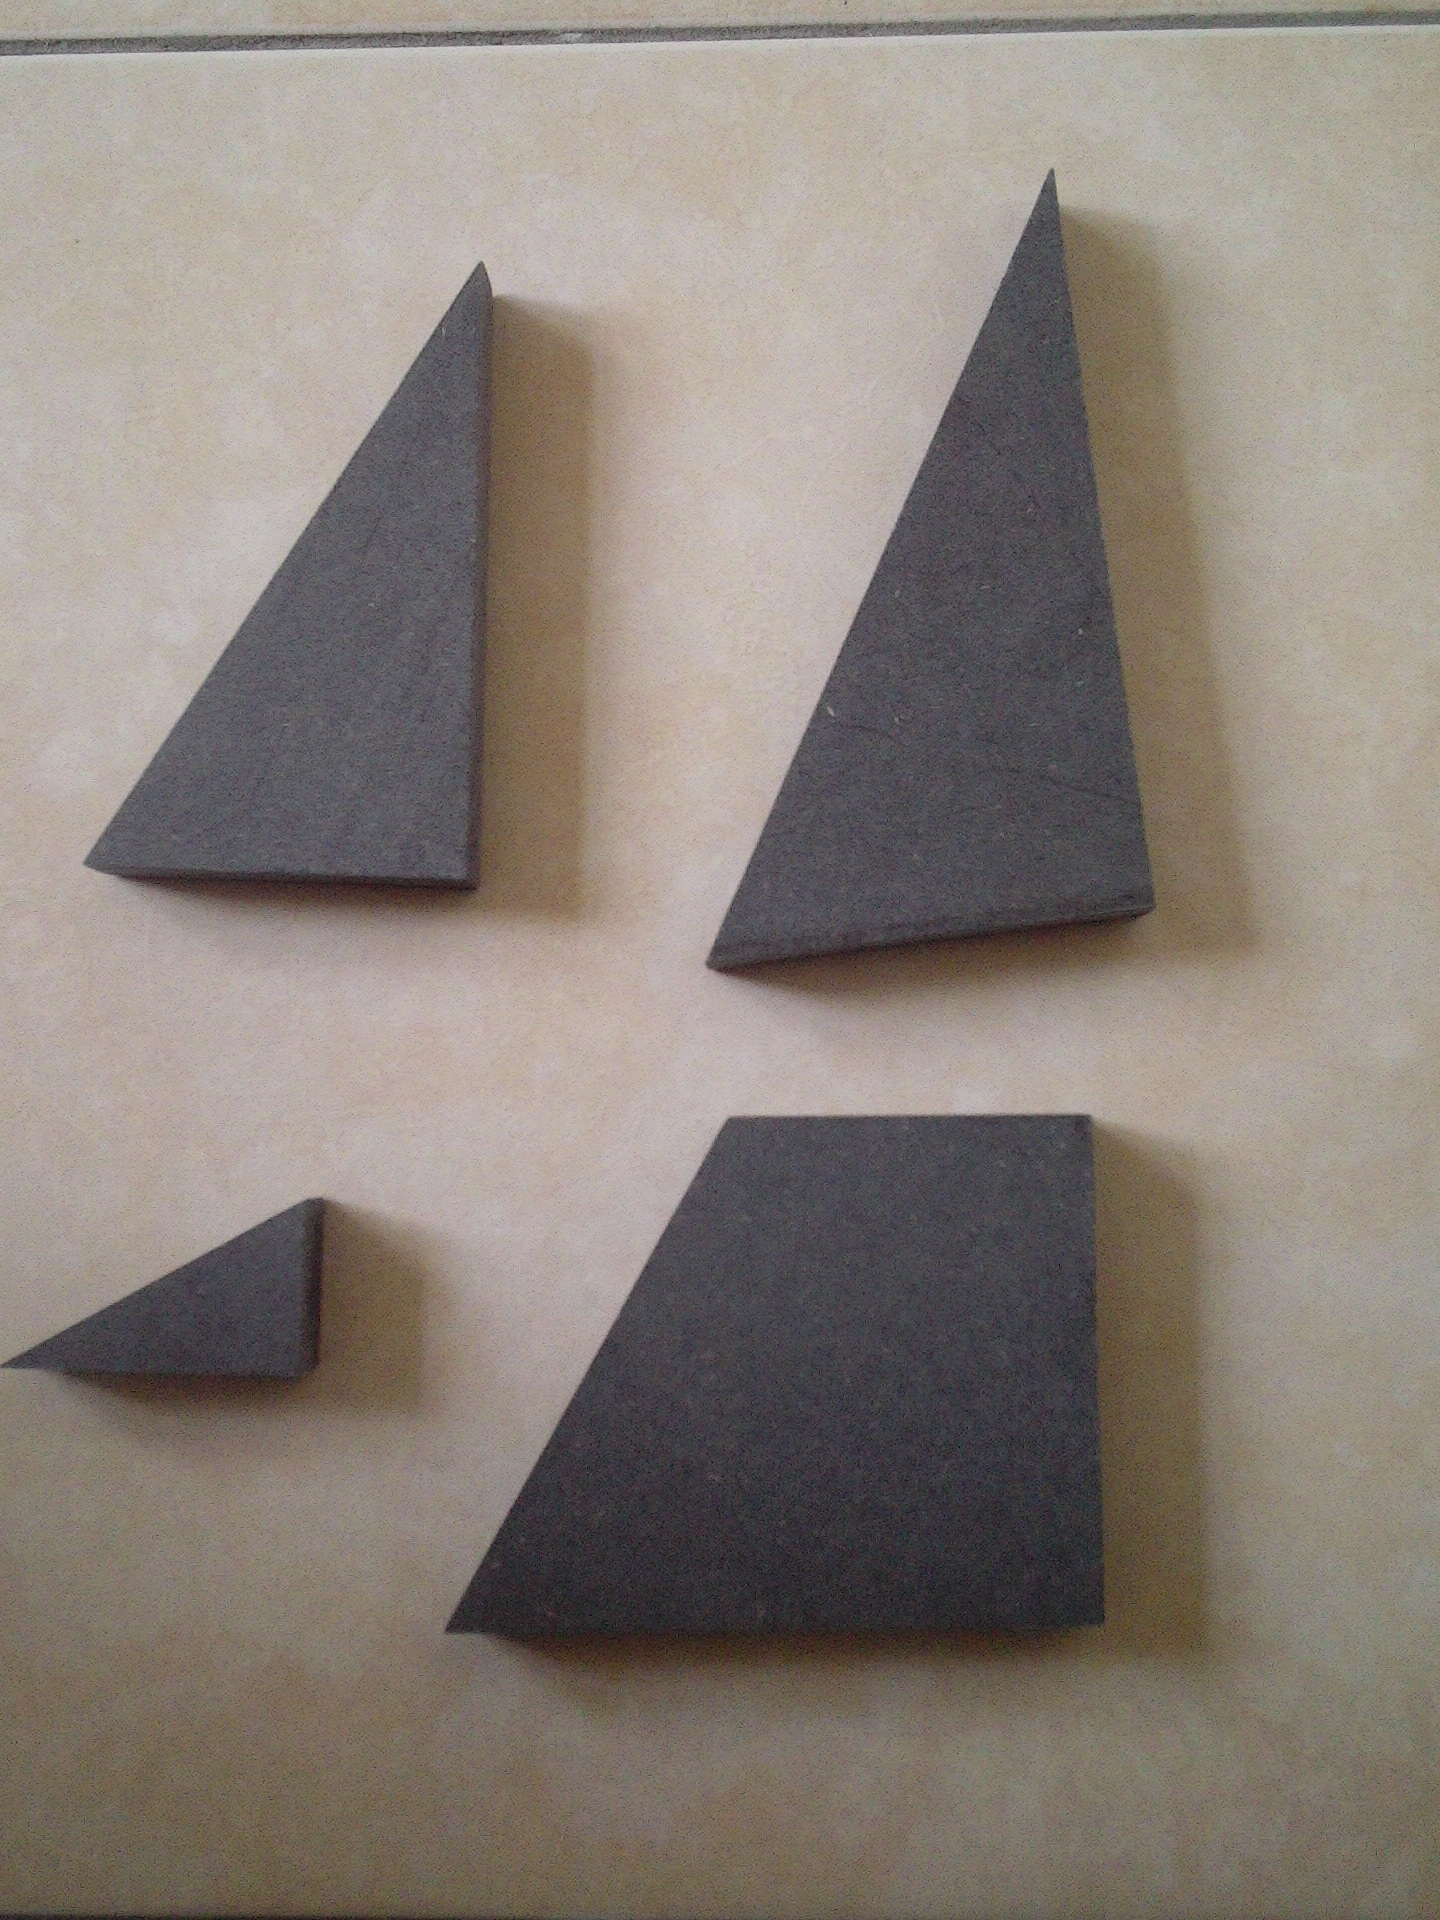
\includegraphics[height=5cm]{PIC0135}
    \label{fig:driehoekpuzzelen}
  }
  \subfloat[]{
    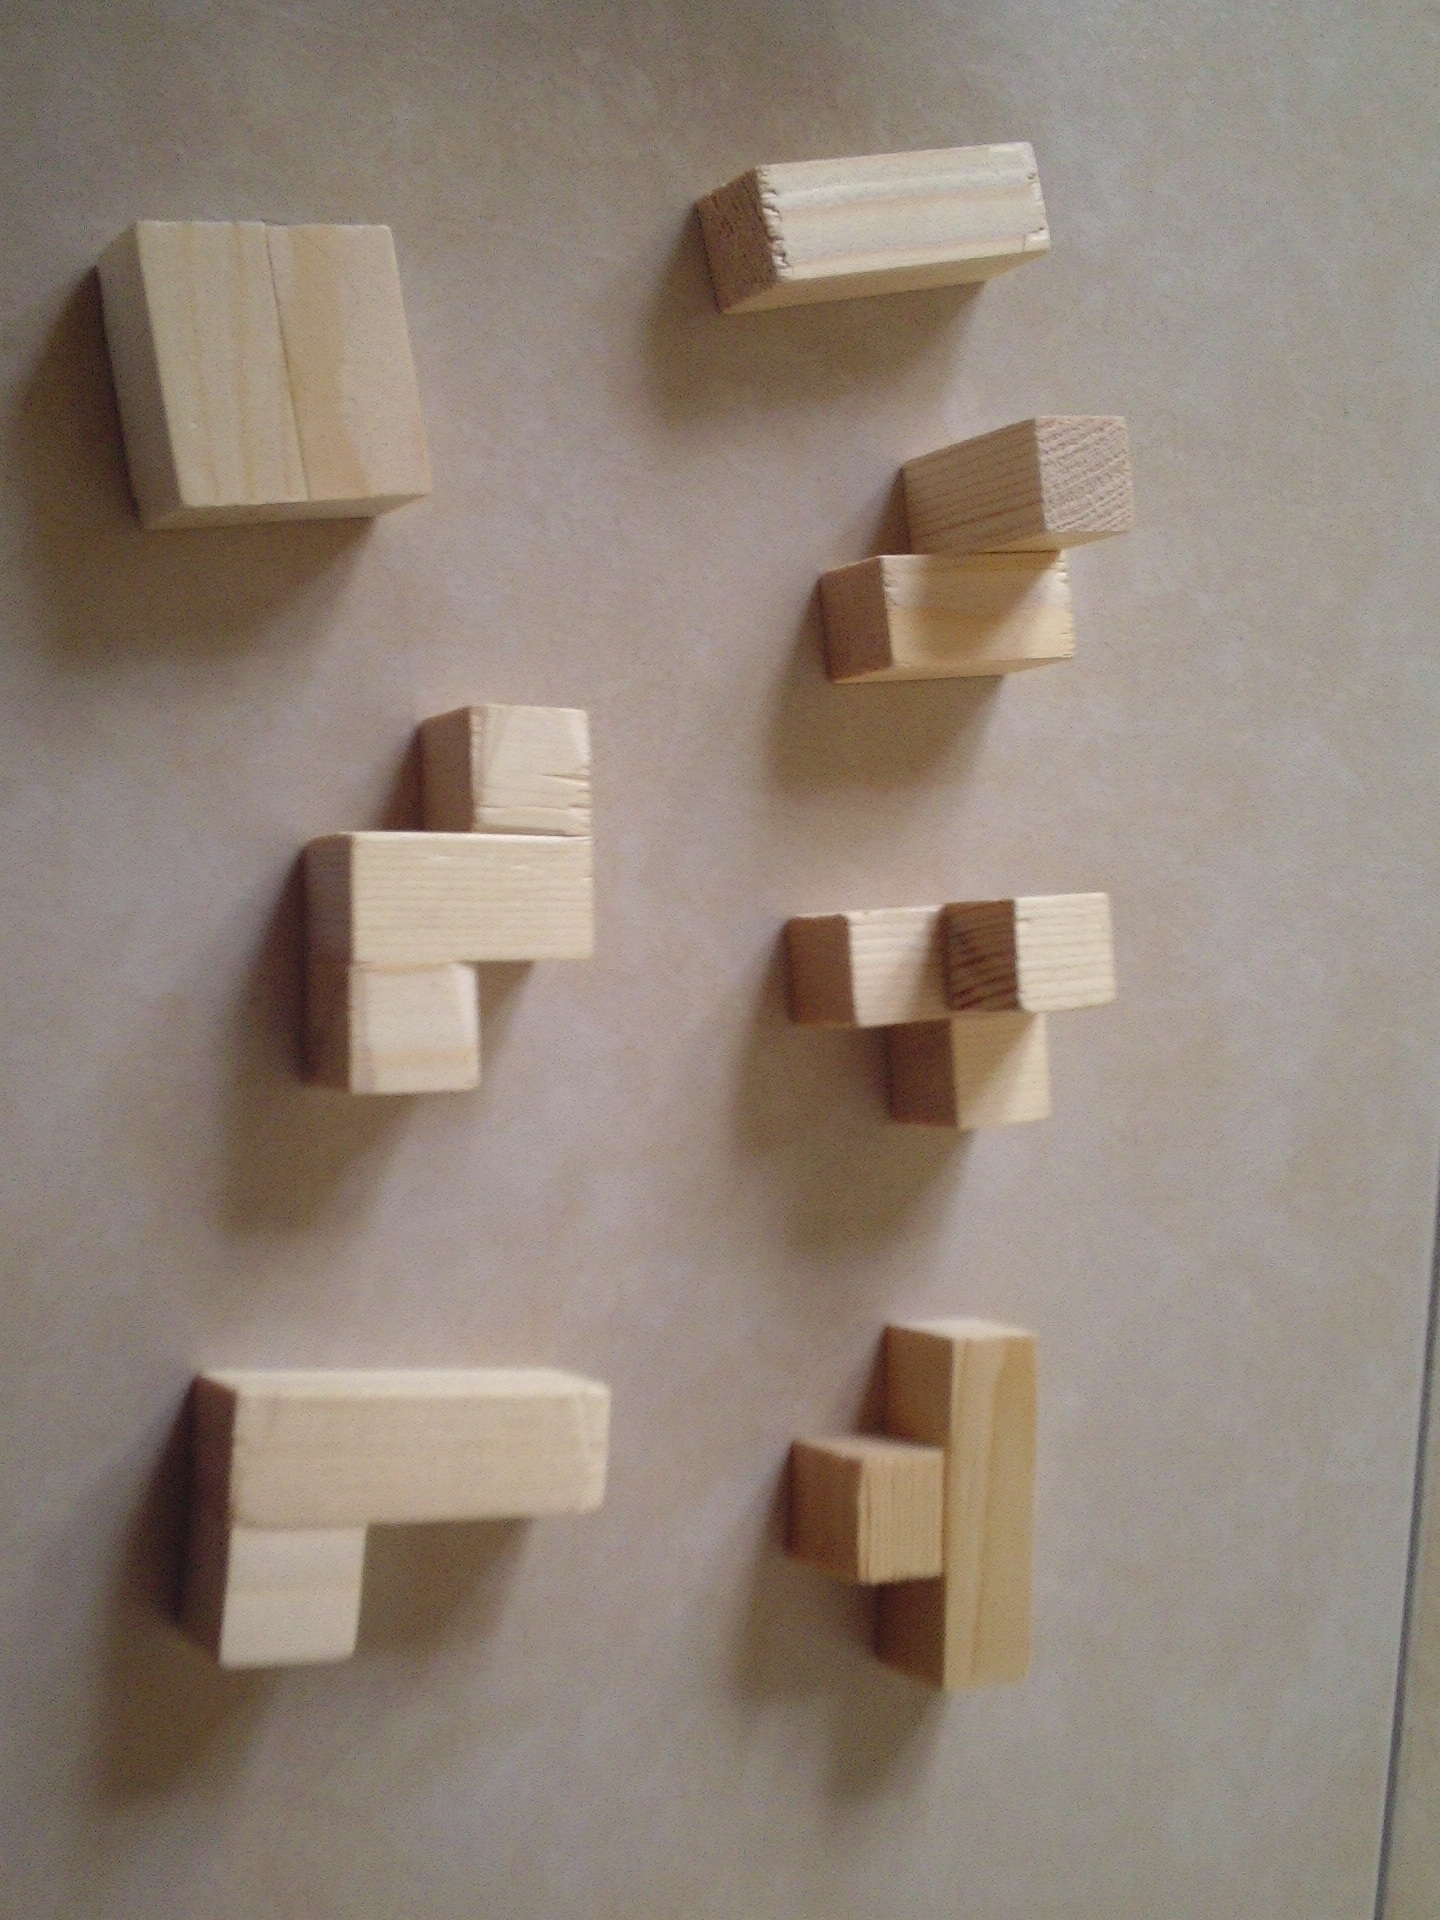
\includegraphics[height=5cm]{PIC0137}
    \label{fig:kubuspuzzelen}
  }
  \caption{Puzzelen van een driehoek en een kubus.}
\end{figure}

\task{Leg de blokken uit Figuur \ref{fig:driehoekpuzzelen} zodat je een vierkant krijgt.}

\task{Leg deze blokken uit Figuur \ref{fig:kubuspuzzelen} zodat je een kubus krijgt.}

\begin{figure}[ht]
  \centering
  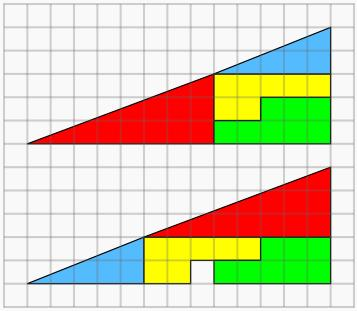
\includegraphics[height=5cm]{driehoek1}
  \caption{Driehoeken met een paradox?}
  \label{fig:driehoekenparadox}
\end{figure}

\ask{Wat is er in Figuur \ref{fig:driehoekenparadox} aan de hand?}

\answer{Bekijk de oppervlaktes van de rode driehoek, de blauwe driehoek en de grote driehoek. Deze laatste is eigenlijk geen driehoek, want als je kijkt naar de verhoudingen van basis en hoogte van de kleine driehoeken, zie je dat er een knik zit in de zogezegde schuine zijde van de grote driehoek. Zie ook \cite{18}.}

\subsection{Wordt vervolgd}
In de volgende les zullen we ons bezighouden met het vullen van vierkanten met vierkanten. Vervolgens zal het betegelen van een vlak met zeshoeken de leidraad zijn bij het vullen van een gegeven vlak.

\teacher{In de eerstkomende lessen zullen we het hebben over complete vlakvullingen (les over vierkanten vullen met vierkanten en perfecte vierkanten en de les over de meetkundige interpretaties van kwadratische vergelijkingen en kubische vergelijkingen).}

\clearpage
